% ++++++++++++++++++++++++++++++++++++++++
% Don't modify this section unless you know what you're doing!
\documentclass[a4paper,12pt]{article}
\usepackage{tabularx} % extra features for tabular environment
\usepackage{amsmath}  % improve math presentation
\usepackage{graphicx} % takes care of graphic including machinery
\usepackage[margin=0.75in]{geometry} % decreases margins
\usepackage{verbatim}
\usepackage{float}
\usepackage{hyperref}
\hypersetup{
	colorlinks=true,       % false: boxed links; true: colored links
	linkcolor=black,        % color of internal links
	citecolor=blue,        % color of links to bibliography
	filecolor=magenta,     % color of file links
	urlcolor=blue         
}
%++++++++++++++++++++++++++++++++++++++++
\setlength{\parindent}{0pt}
\setlength\parskip{1em plus 0.1em minus 0.2em}

\begin{document}
\title{%
Currents in LCR \\
\large PHY224 Lab 7}
\author{Fredrik Dahl Bråten, Pankaj Patil}
\date{\today}
\maketitle
%\tableofcontents


\begin{center}
	\section*{Abstract}
	Test 2
	sheetal.jain@mail.utoronto.ca
\end{center}

\section{Introduction}


\section{Methods, Materials and Experimental Procedure}

We successfully followed the procedures as described by the TA and lab manual \cite{lab-manual-ex7} for this experiment.

\section{Results}



\section{Discussion}

\section{Conclusions}

\pagebreak

\appendix

\section{Appendix}

\subsection{Oscilloscope Readings}

\begin{figure}[H]
  \centering
  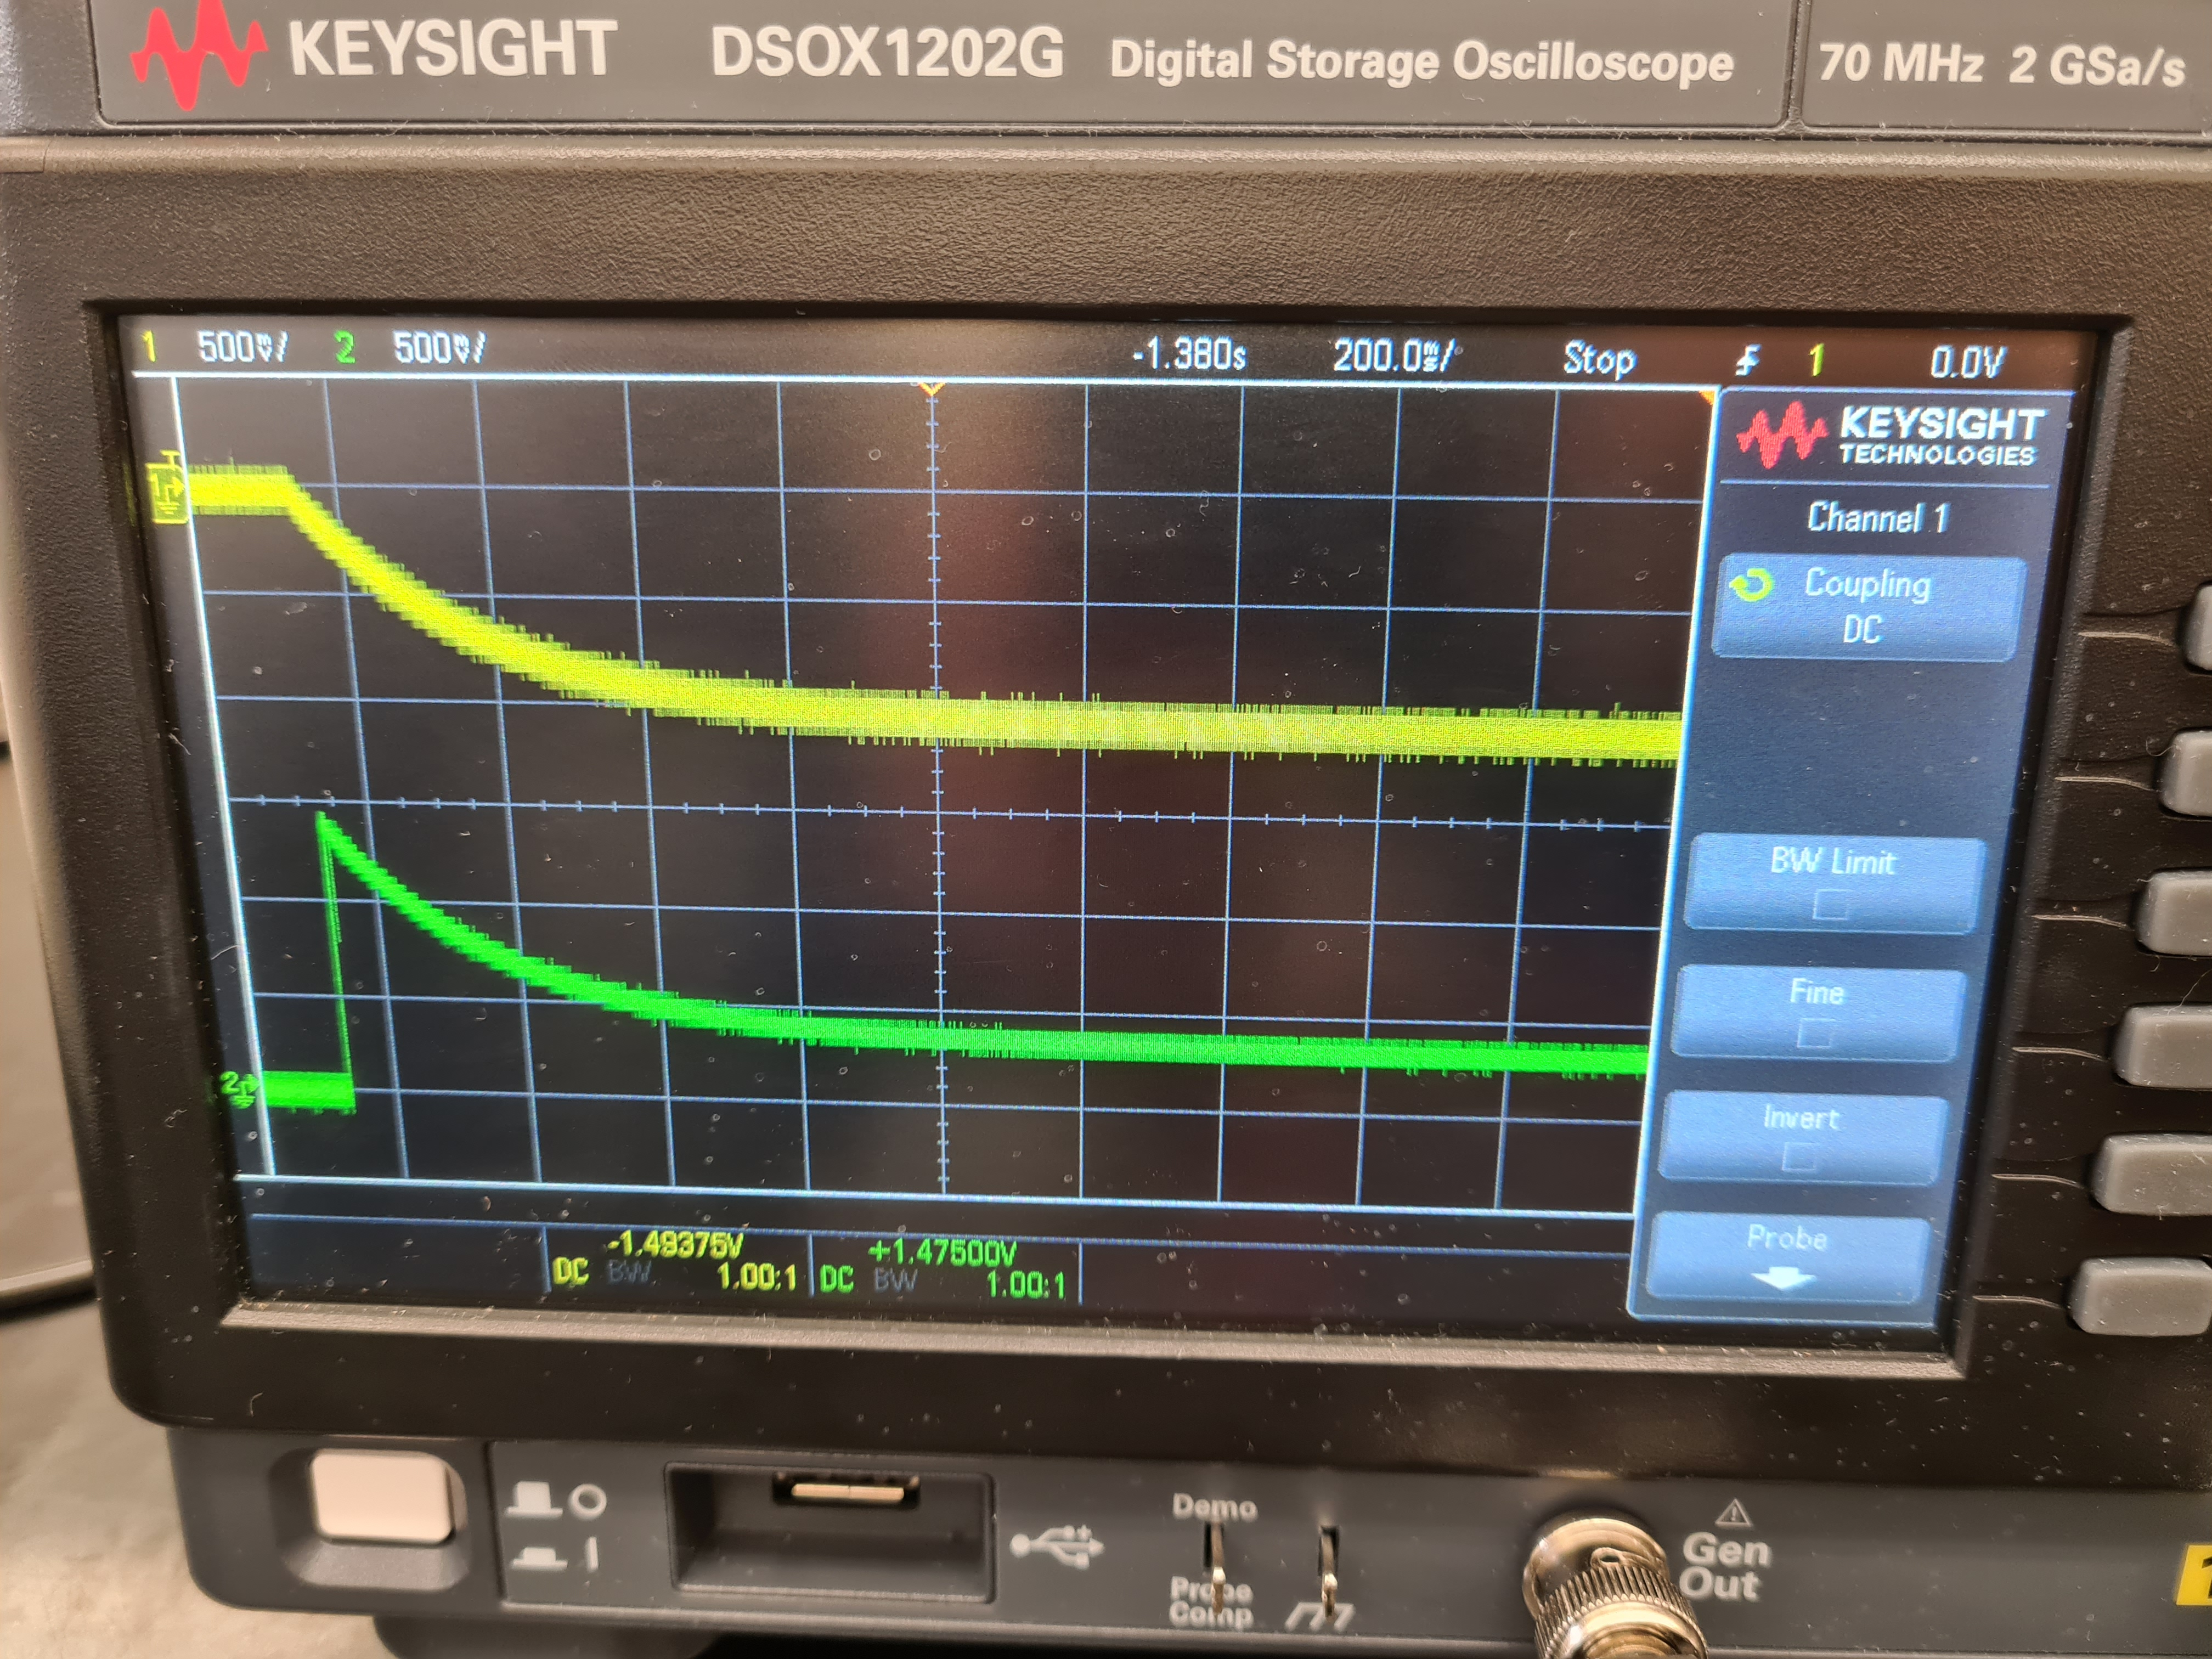
\includegraphics[width=1.0\linewidth]{../data/20211116_101002.jpg}    
  \begin{center}
    \begin{center}   
    \end{center}  \end{center}
  \caption{Oscilloscope Reading (Peak to Peak Alignment)}
  \label{osc}
\end{figure}

\begin{figure}[H]
  \centering
  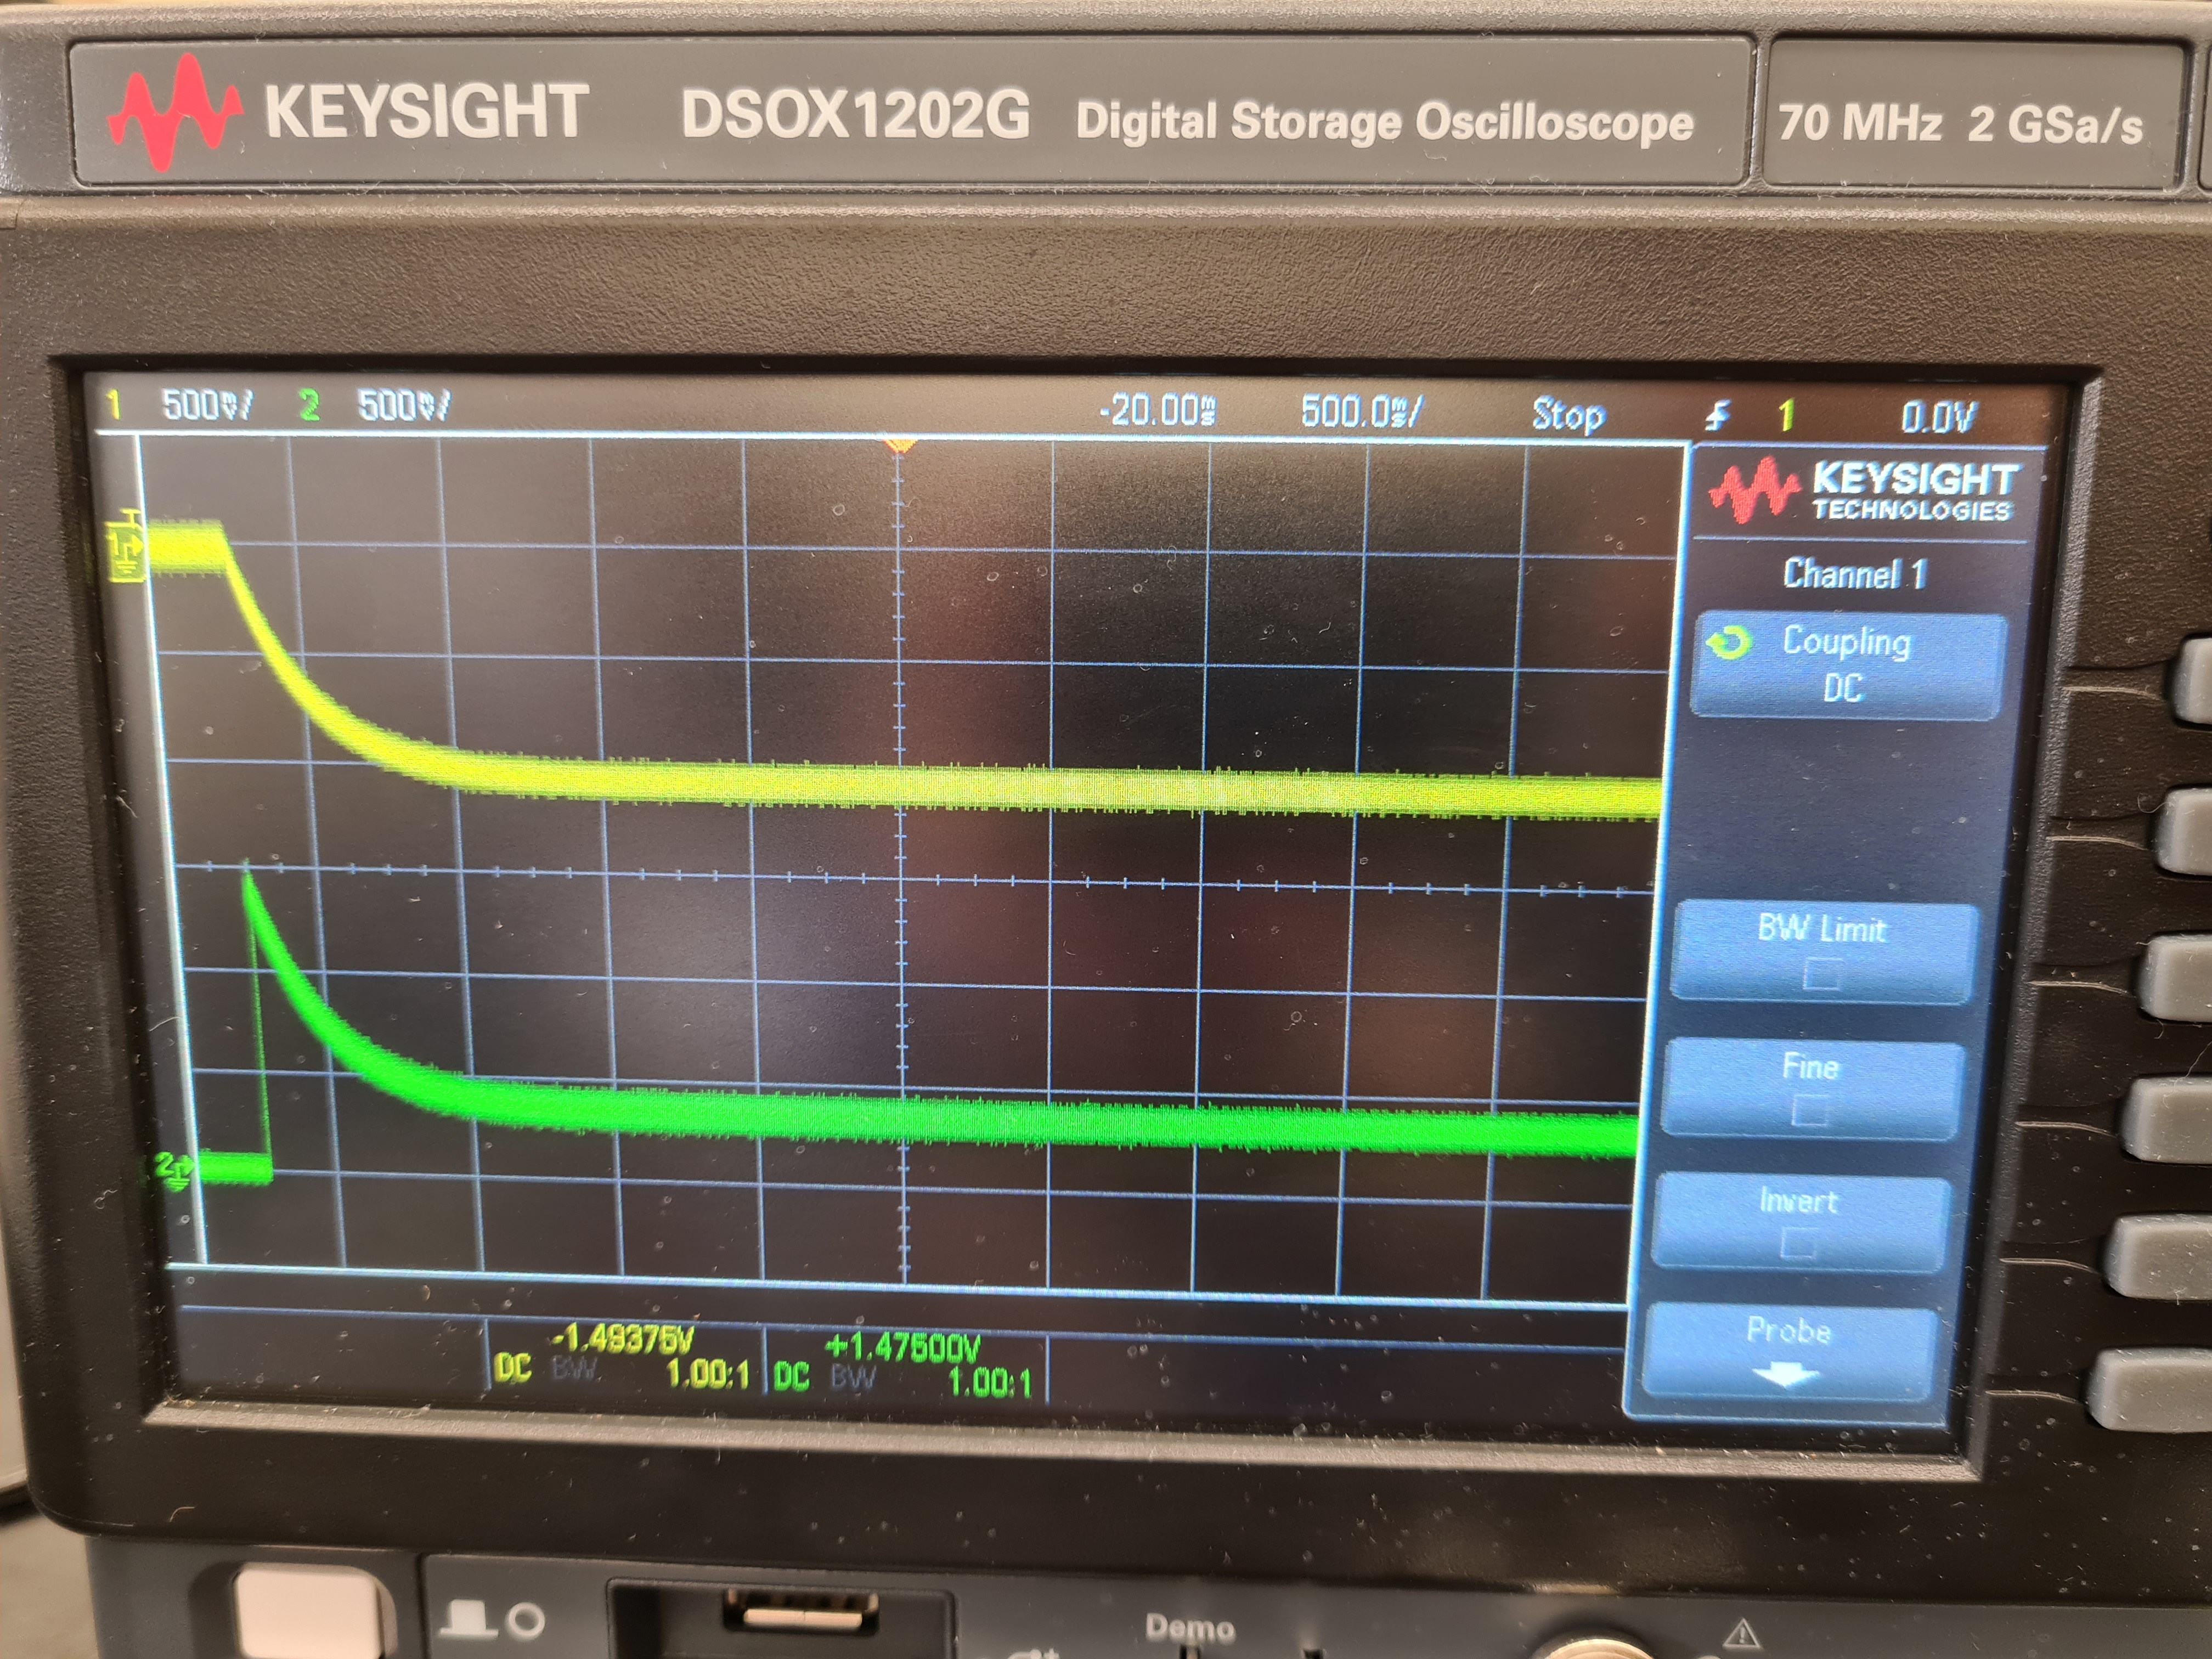
\includegraphics[width=1.0\linewidth]{../data/20211116_101233.jpg}    
  \begin{center}
    \begin{center}   
    \end{center}  \end{center}
  \caption{Oscilloscope Reading (Peak to Peak Alignment)}
  \label{osc}
\end{figure}

\begin{figure}[H]
  \centering
  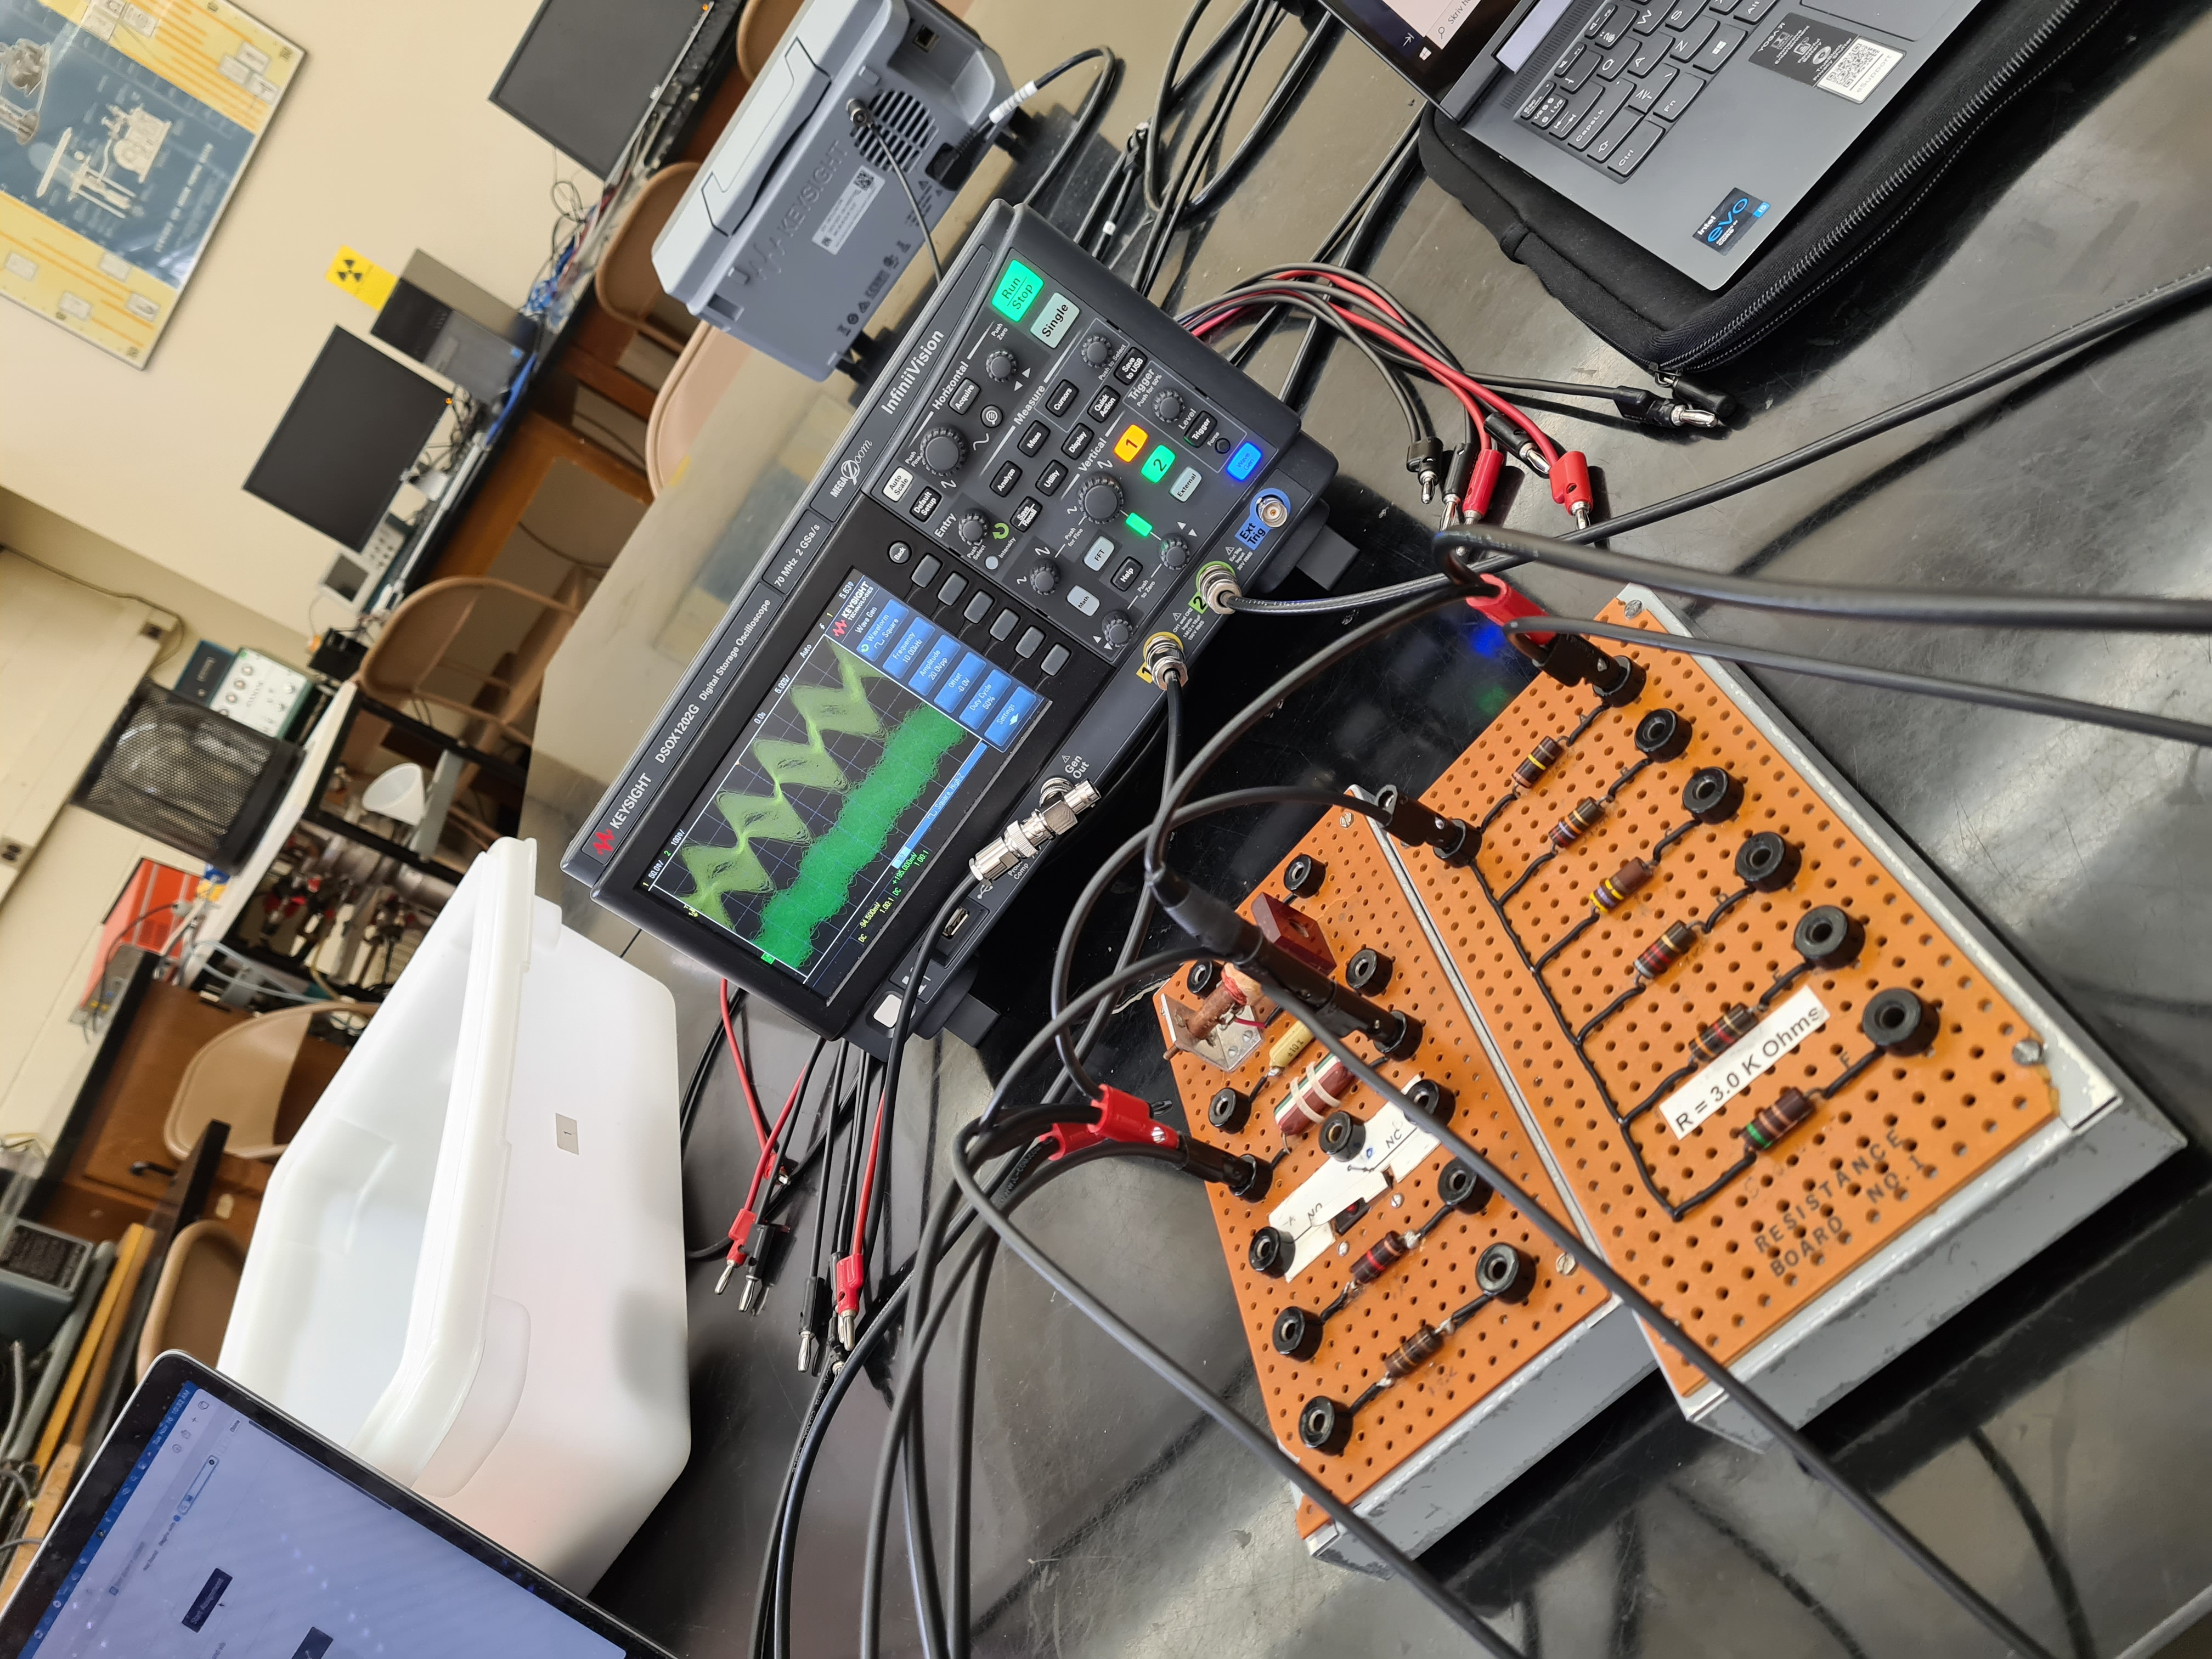
\includegraphics[width=1.0\linewidth]{../data/20211116_103322.jpg}    
  \begin{center}
    \begin{center}   
    \end{center}  \end{center}
  \caption{Oscilloscope Reading (Peak to Peak Alignment)}
  \label{osc}
\end{figure}

\begin{figure}[H]
  \centering
  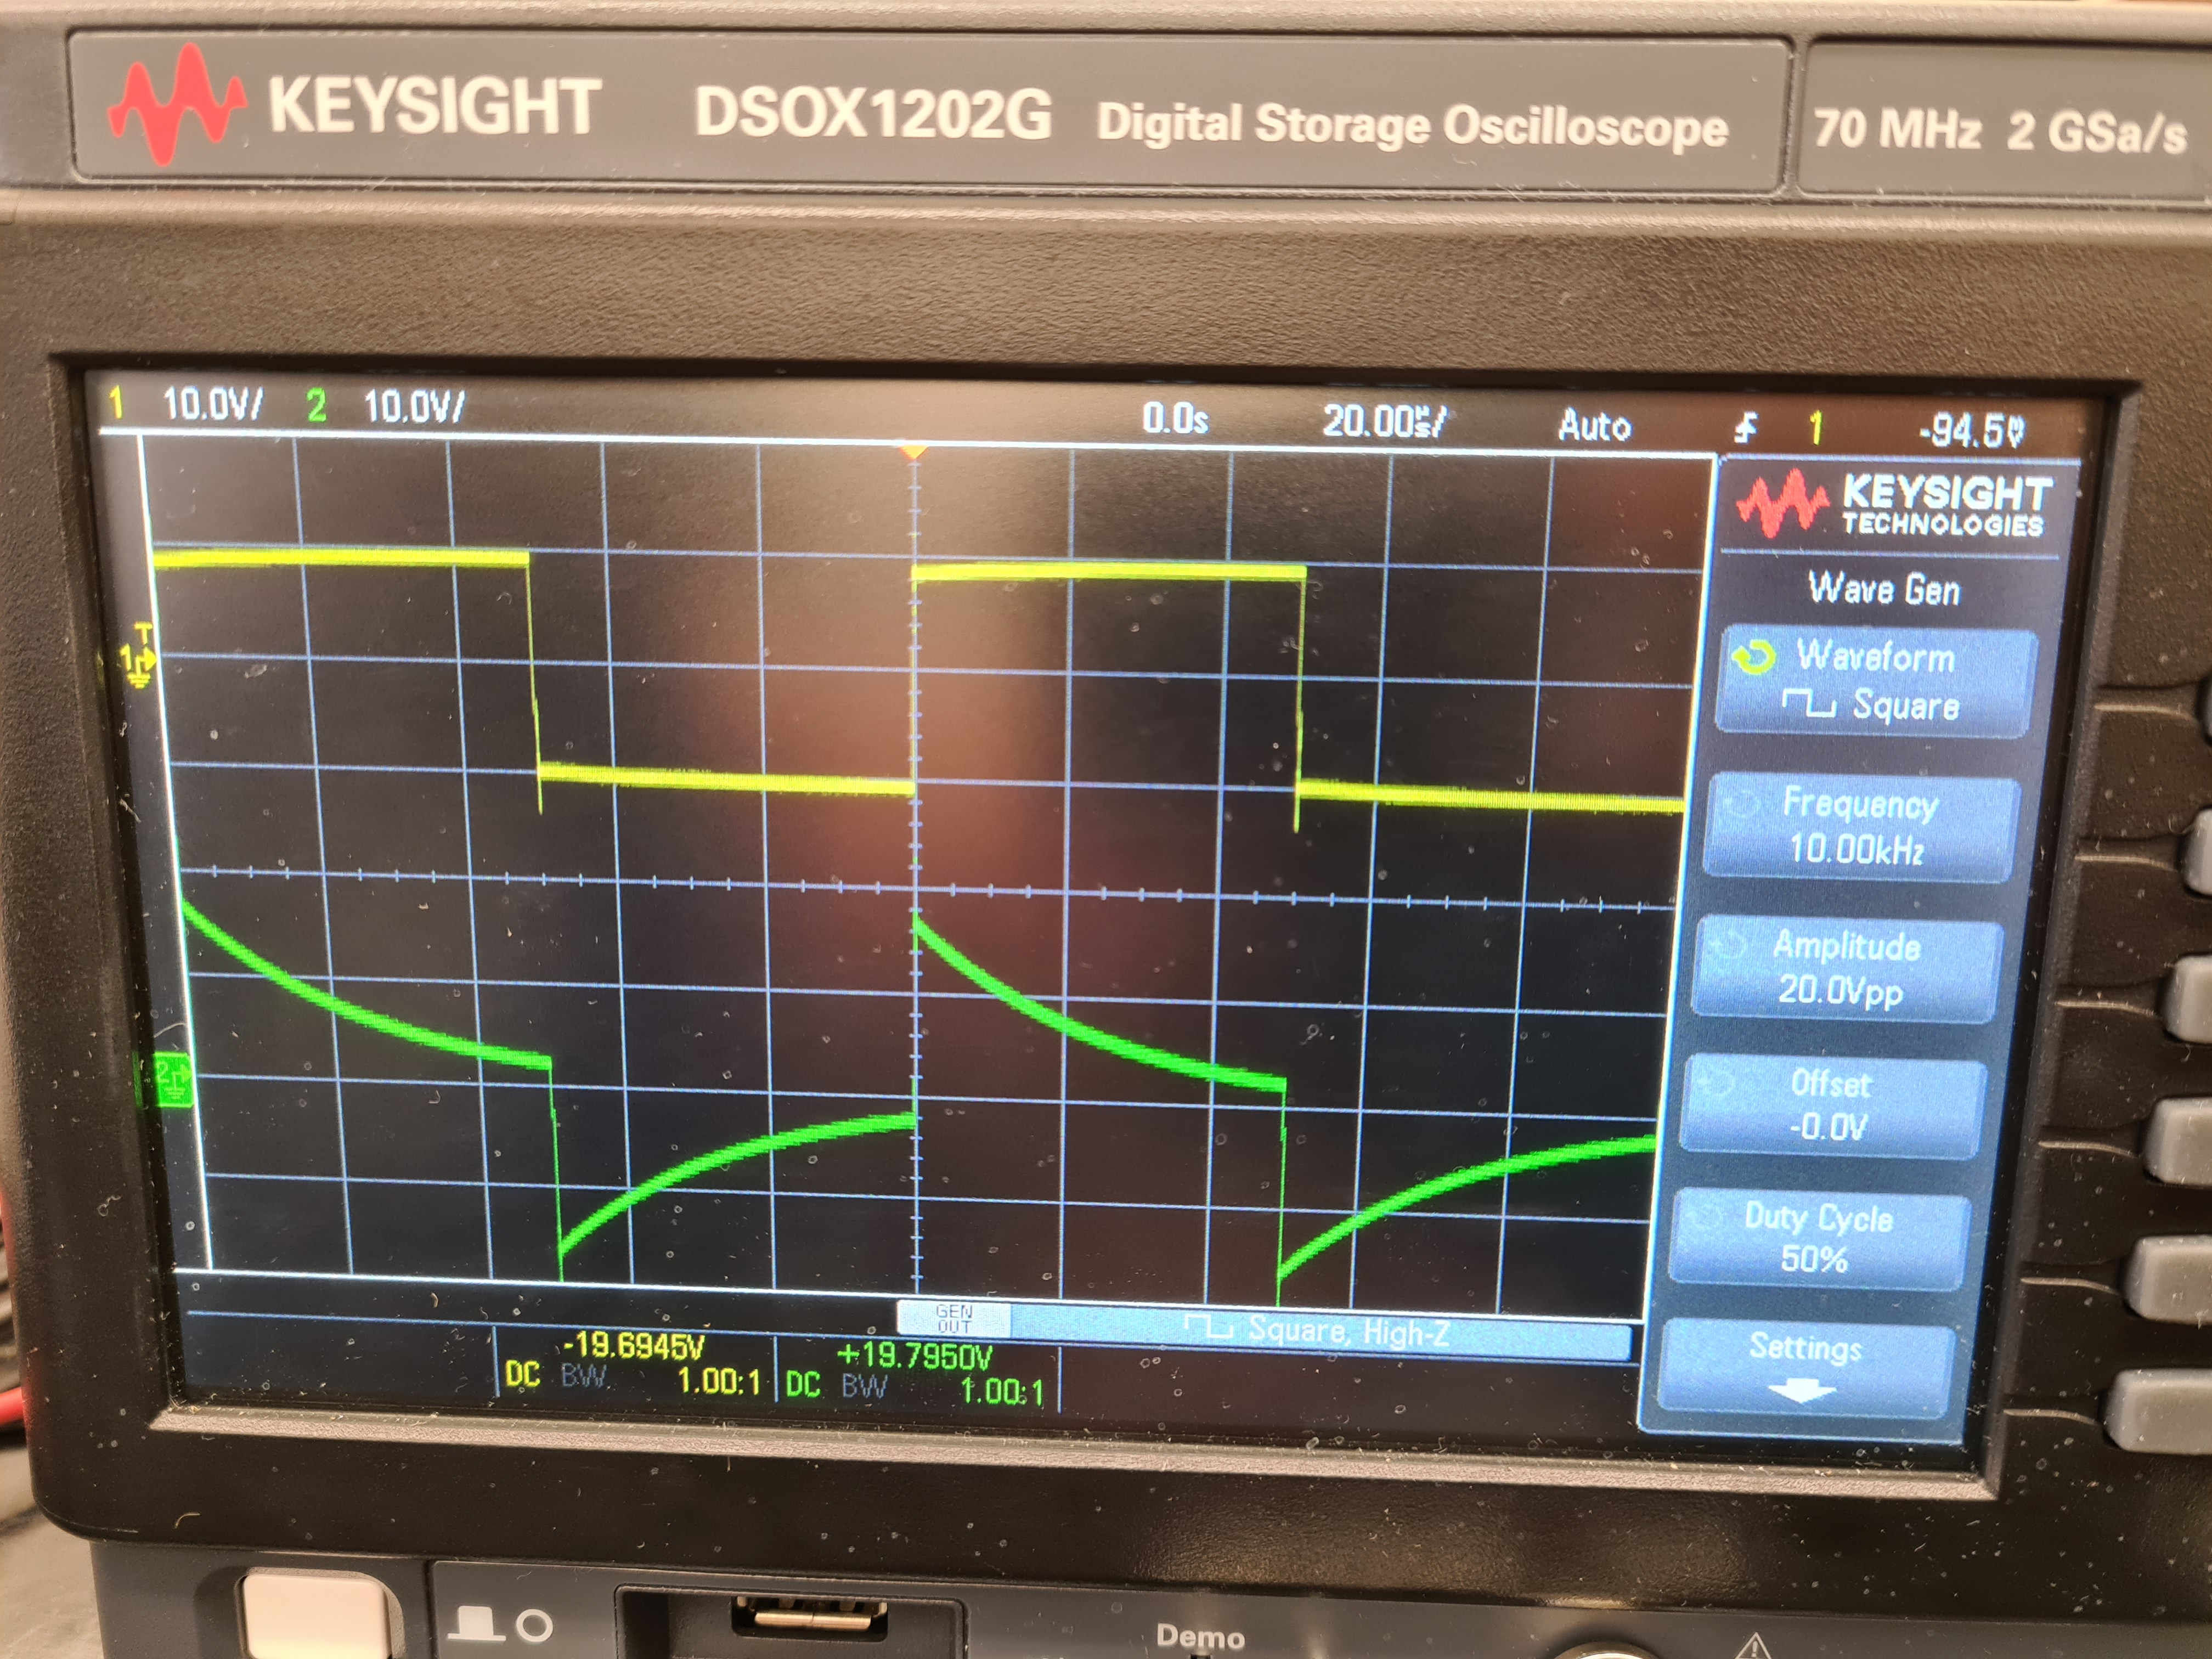
\includegraphics[width=1.0\linewidth]{../data/20211116_104029.jpg}    
  \begin{center}
    \begin{center}   
    \end{center}  \end{center}
  \caption{Oscilloscope Reading (Peak to Peak Alignment)}
  \label{osc}
\end{figure}

\begin{figure}[H]
  \centering
  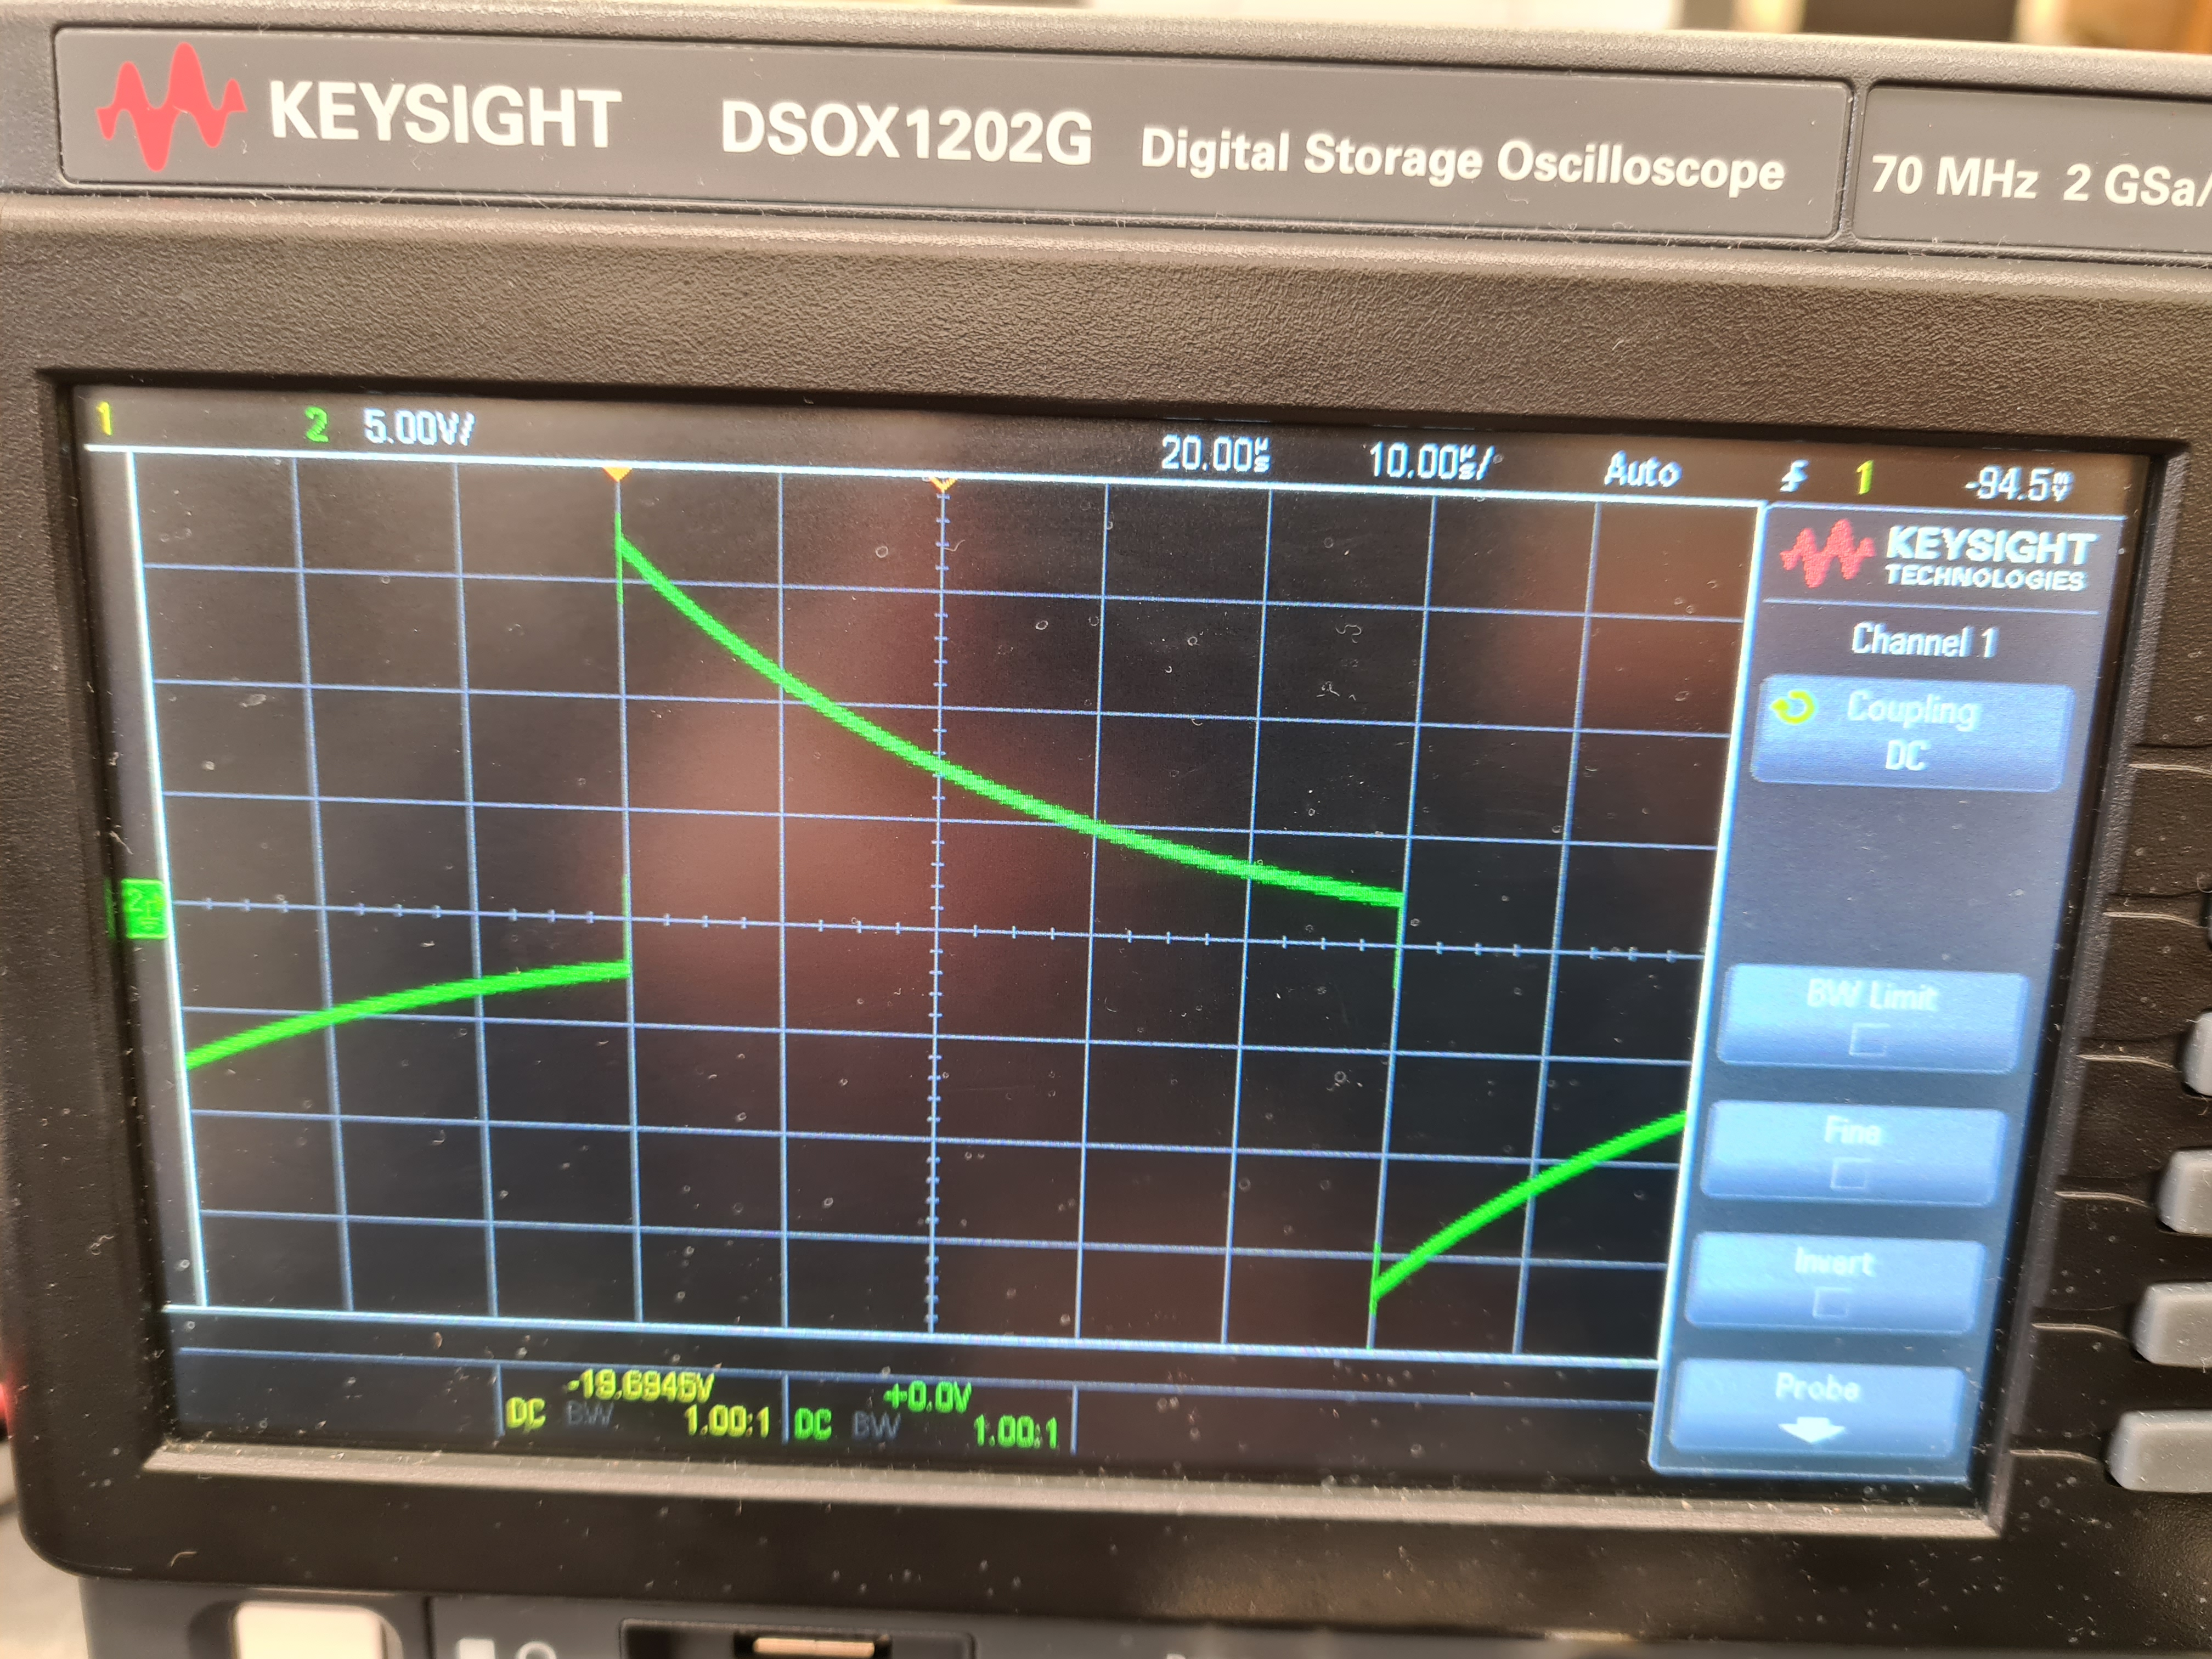
\includegraphics[width=1.0\linewidth]{../data/20211116_104137.jpg}    
  \begin{center}
    \begin{center}   
    \end{center}  \end{center}
  \caption{Oscilloscope Reading (Peak to Peak Alignment)}
  \label{osc}
\end{figure}

\begin{figure}[H]
  \centering
  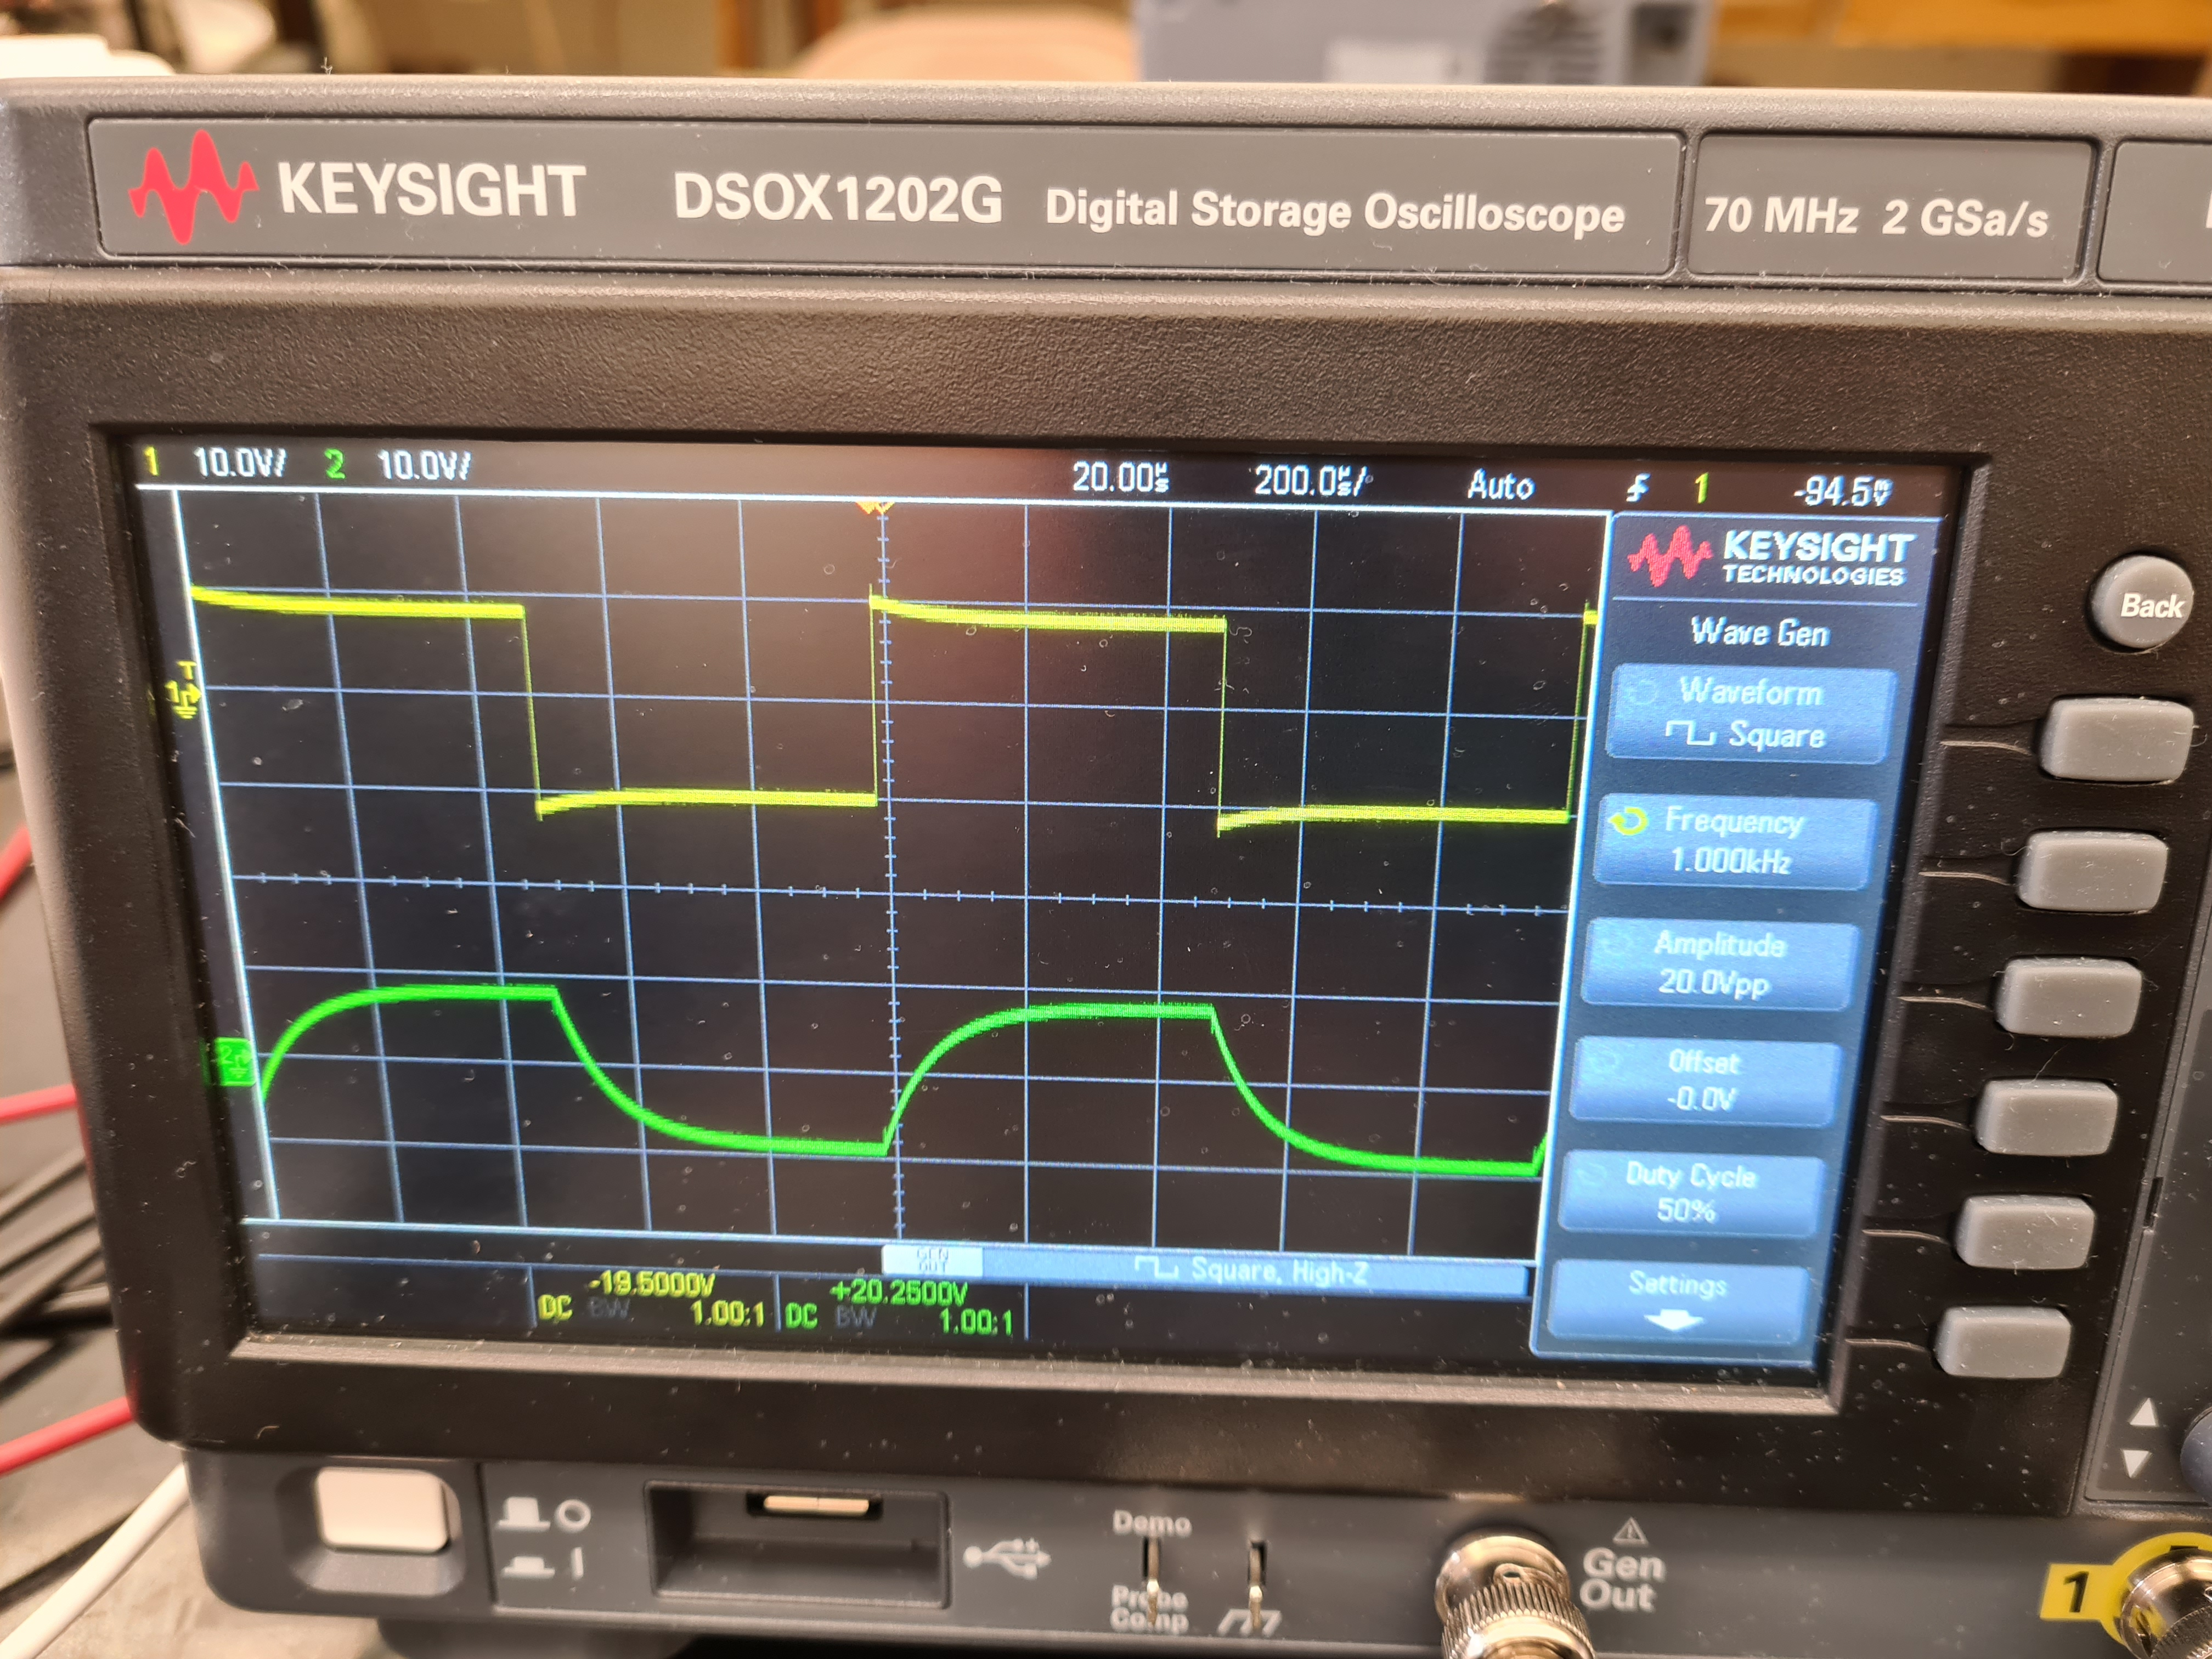
\includegraphics[width=1.0\linewidth]{../data/20211116_104711.jpg}    
  \begin{center}
    \begin{center}   
    \end{center}  \end{center}
  \caption{Oscilloscope Reading (Peak to Peak Alignment)}
  \label{osc}
\end{figure}

\begin{figure}[H]
  \centering
  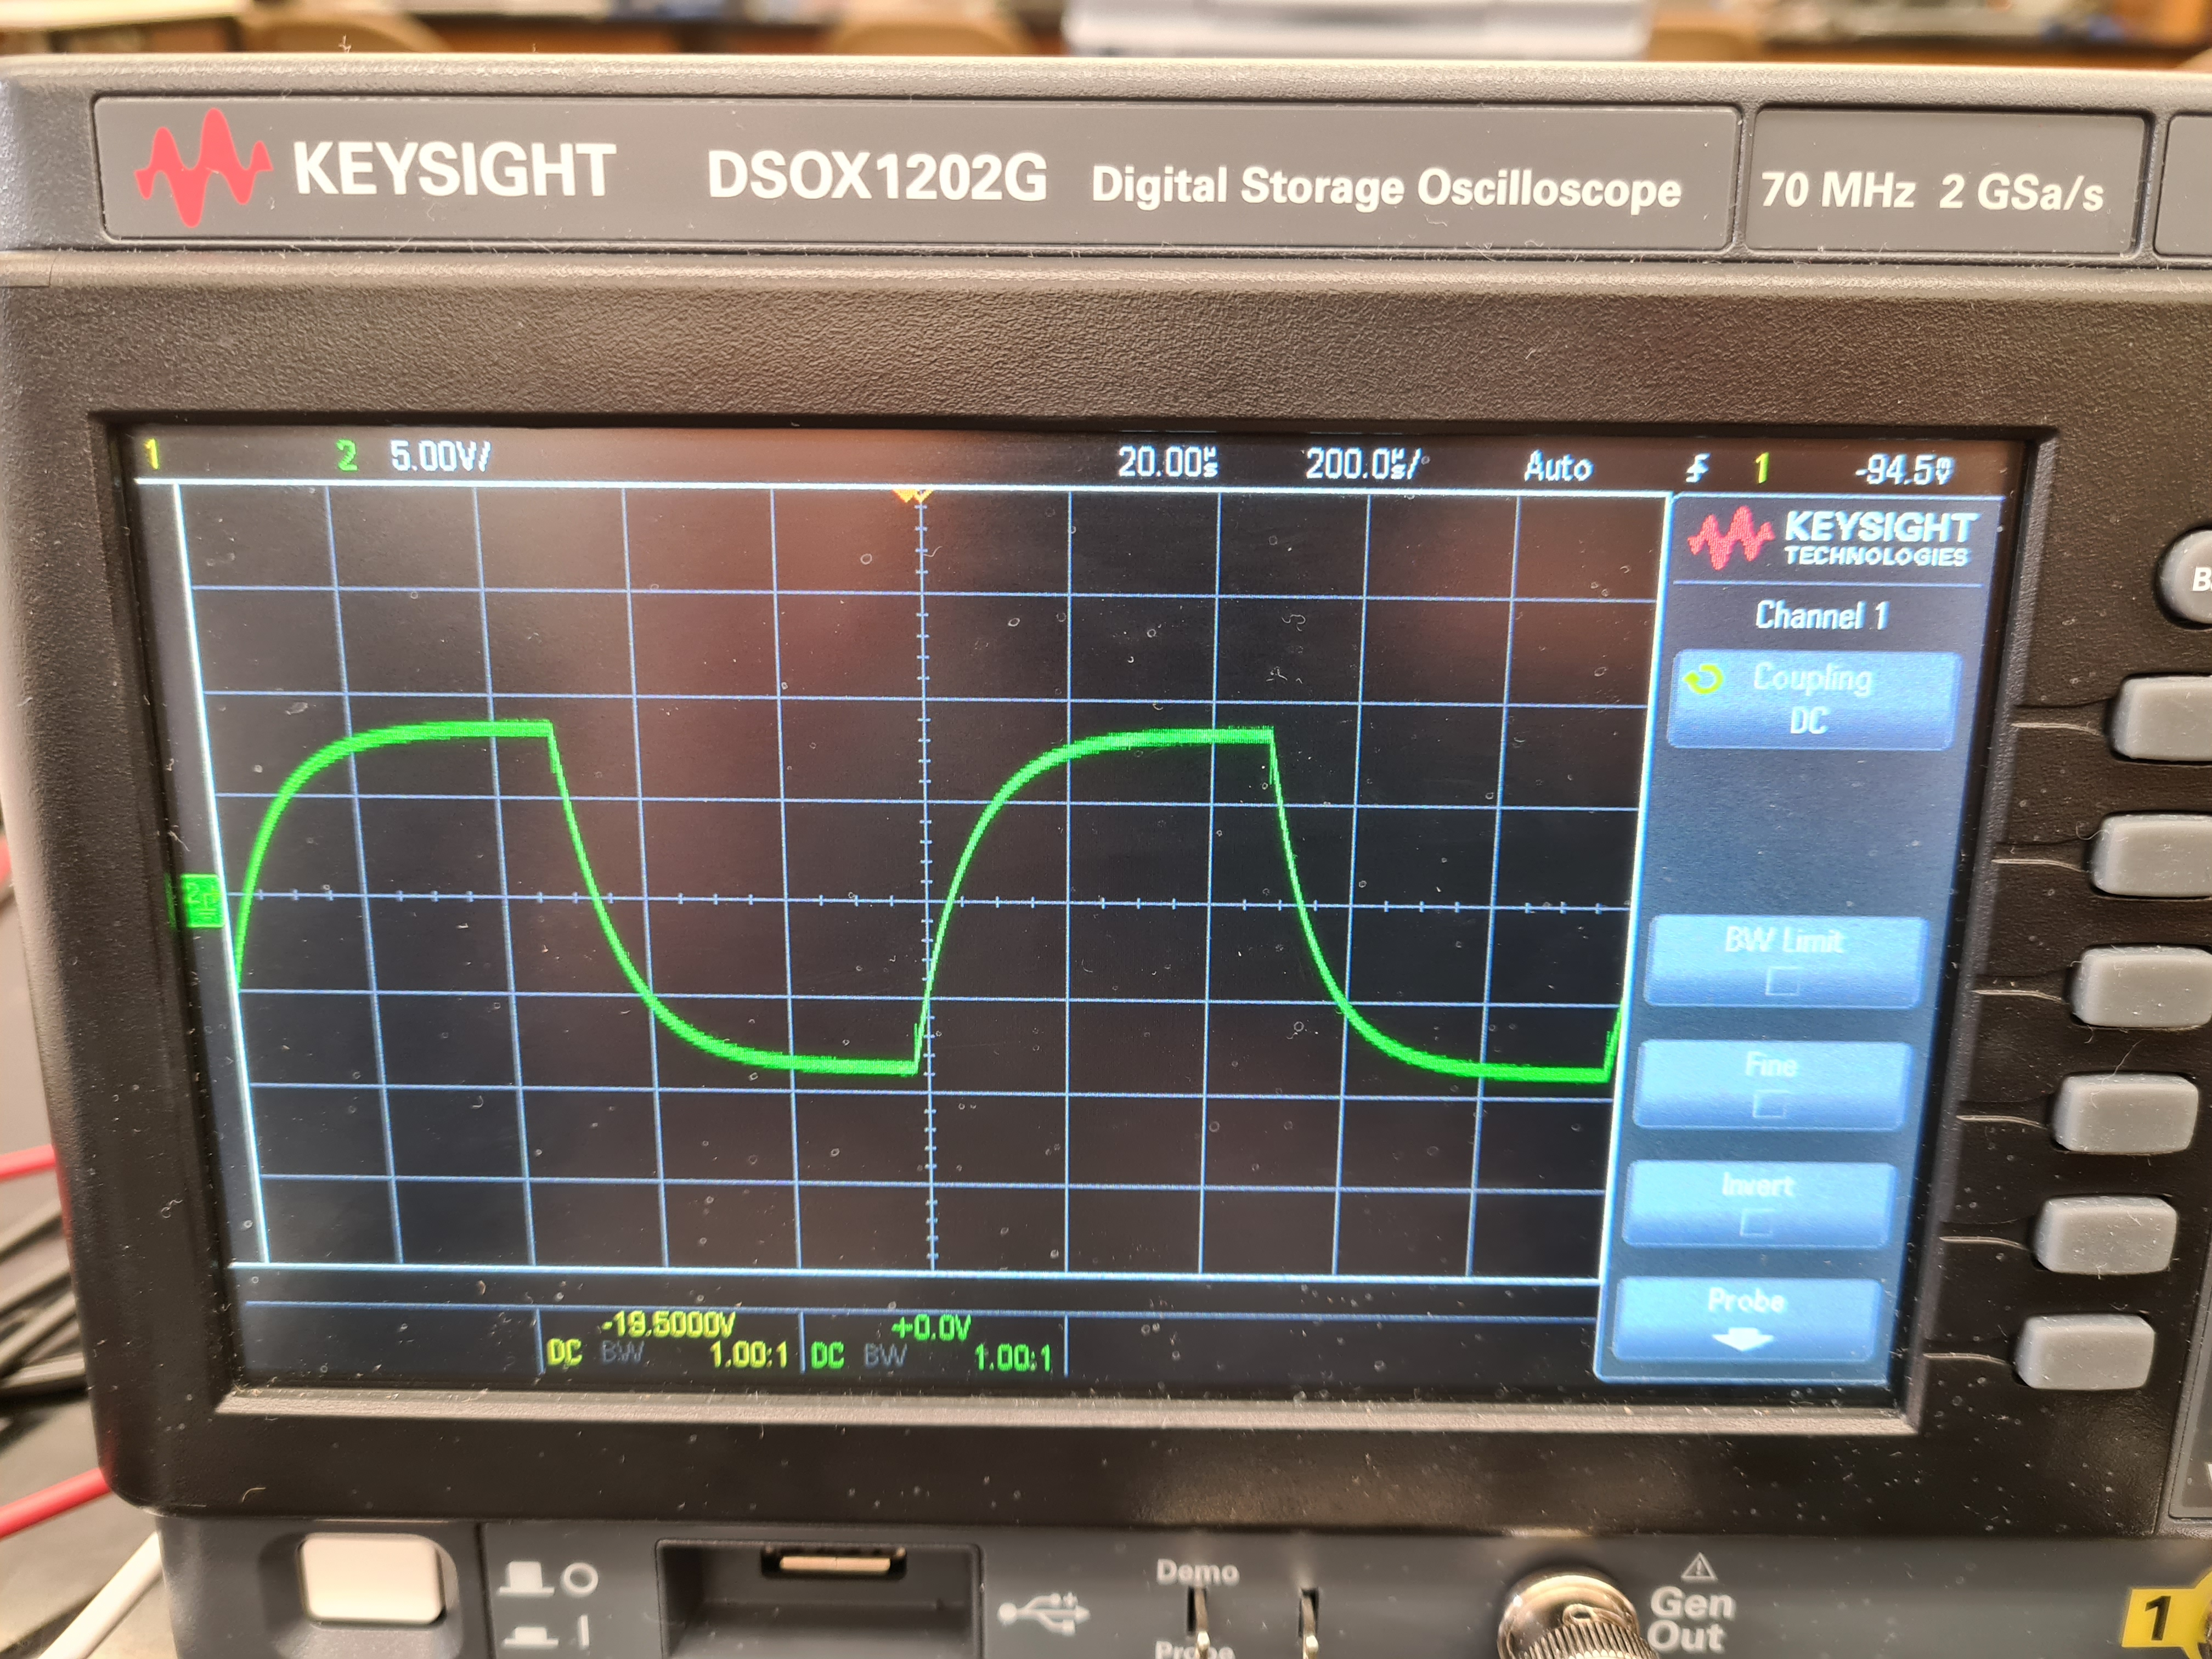
\includegraphics[width=1.0\linewidth]{../data/20211116_104743.jpg}    
  \begin{center}
    \begin{center}   
    \end{center}  \end{center}
  \caption{Oscilloscope Reading (Peak to Peak Alignment)}
  \label{osc}
\end{figure}

\begin{figure}[H]
  \centering
  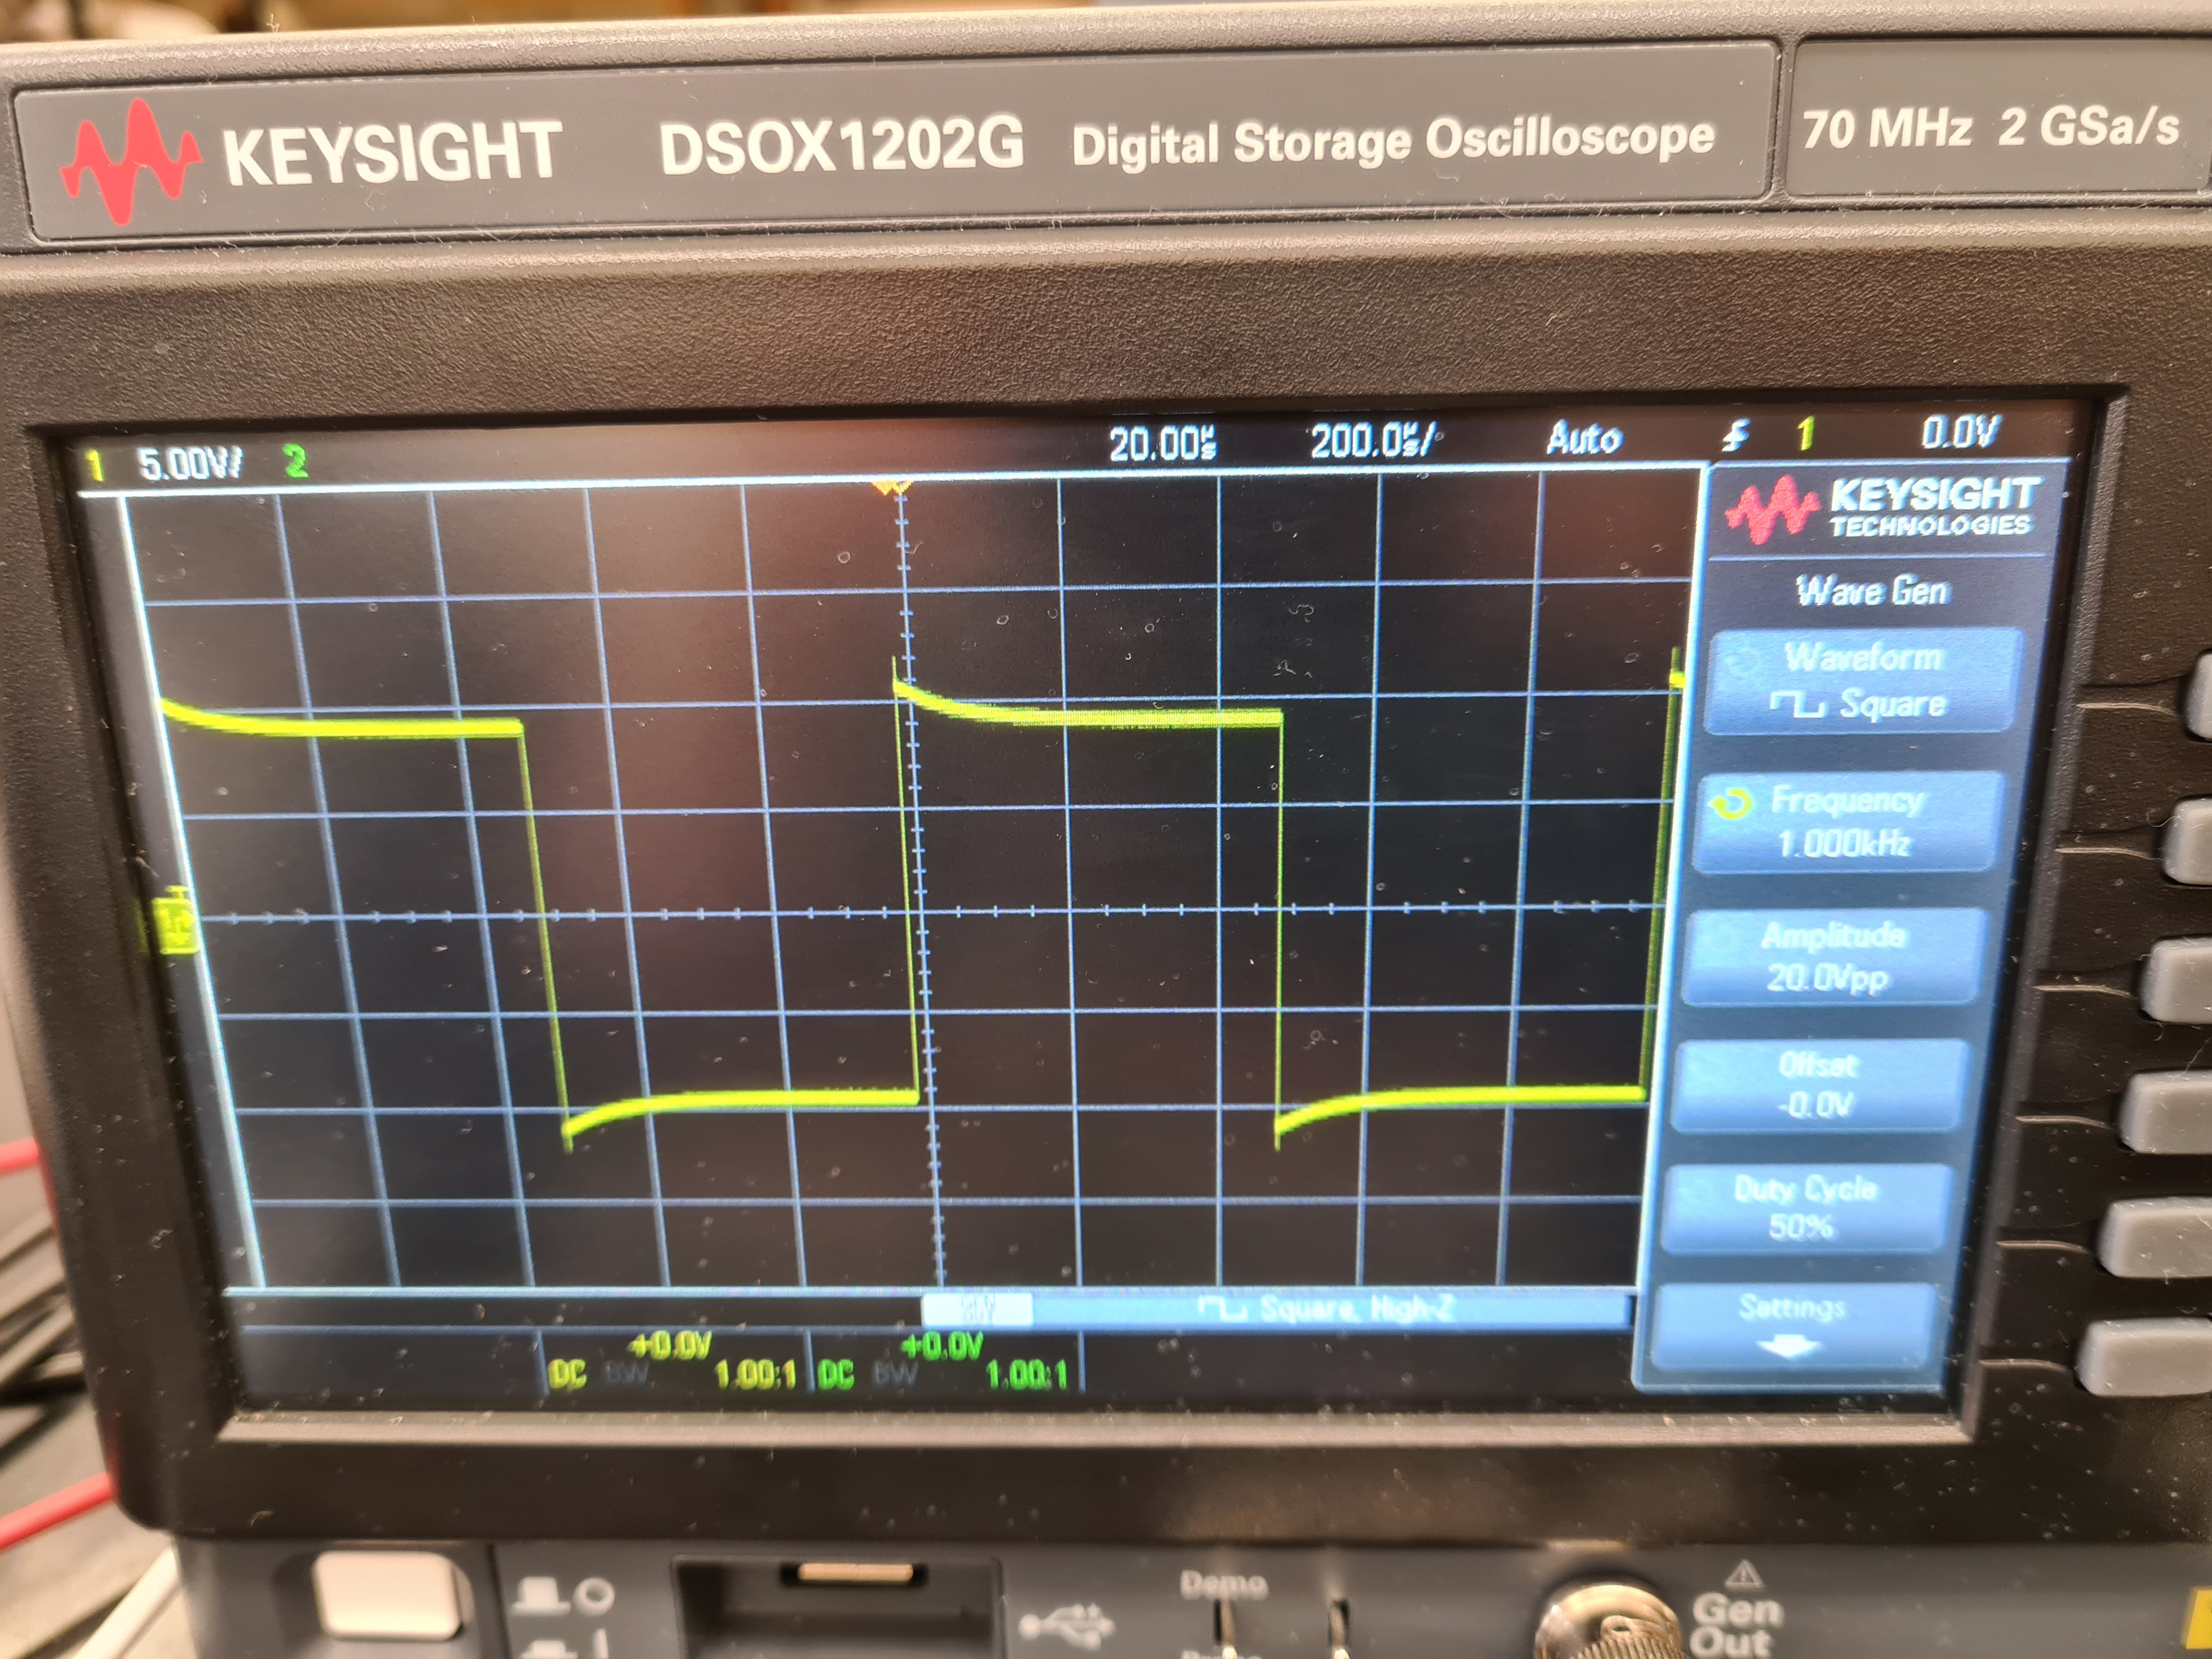
\includegraphics[width=1.0\linewidth]{../data/20211116_104820.jpg}
  \begin{center}
    \begin{center}   
    \end{center}  \end{center}
  \caption{Oscilloscope Reading (Peak to Peak Alignment)}
  \label{osc}
\end{figure}

\begin{figure}[H]
  \centering
  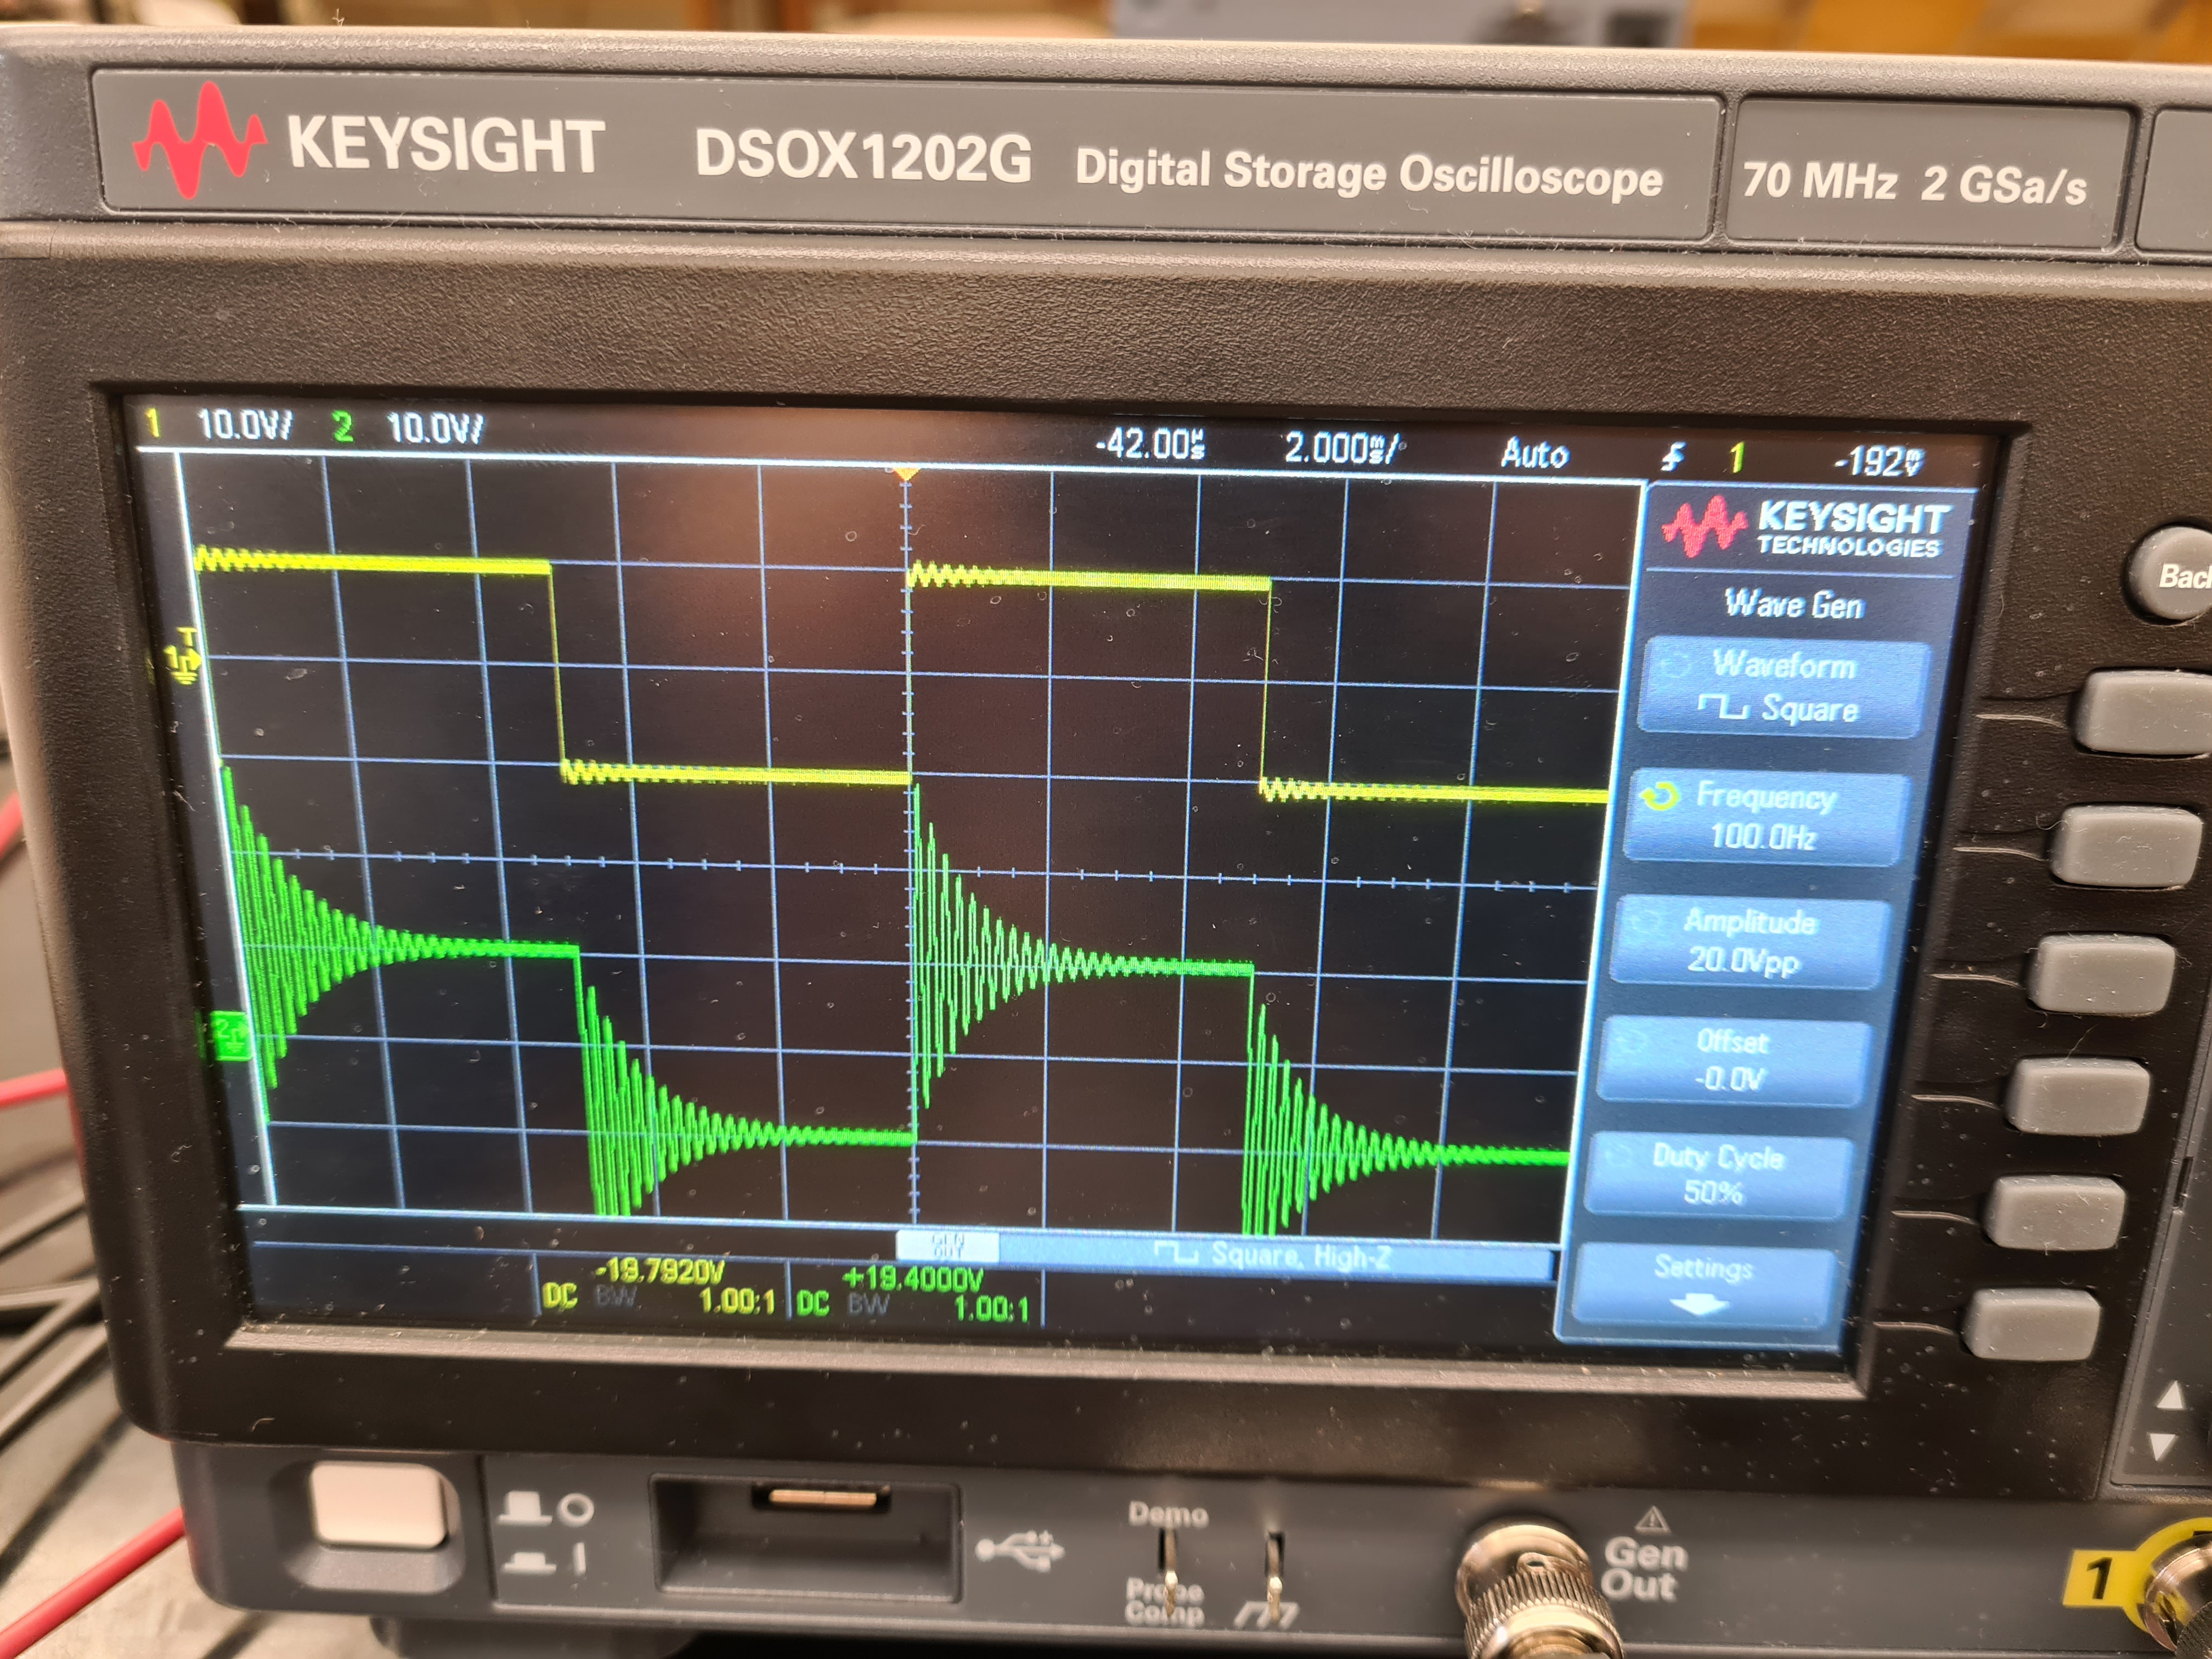
\includegraphics[width=1.0\linewidth]{../data/20211116_110612.jpg}
  \begin{center}
    \begin{center}   
    \end{center}  \end{center}
  \caption{Oscilloscope Reading (Peak to Peak Alignment)}
  \label{osc}
\end{figure}

\begin{figure}[H]
  \centering
  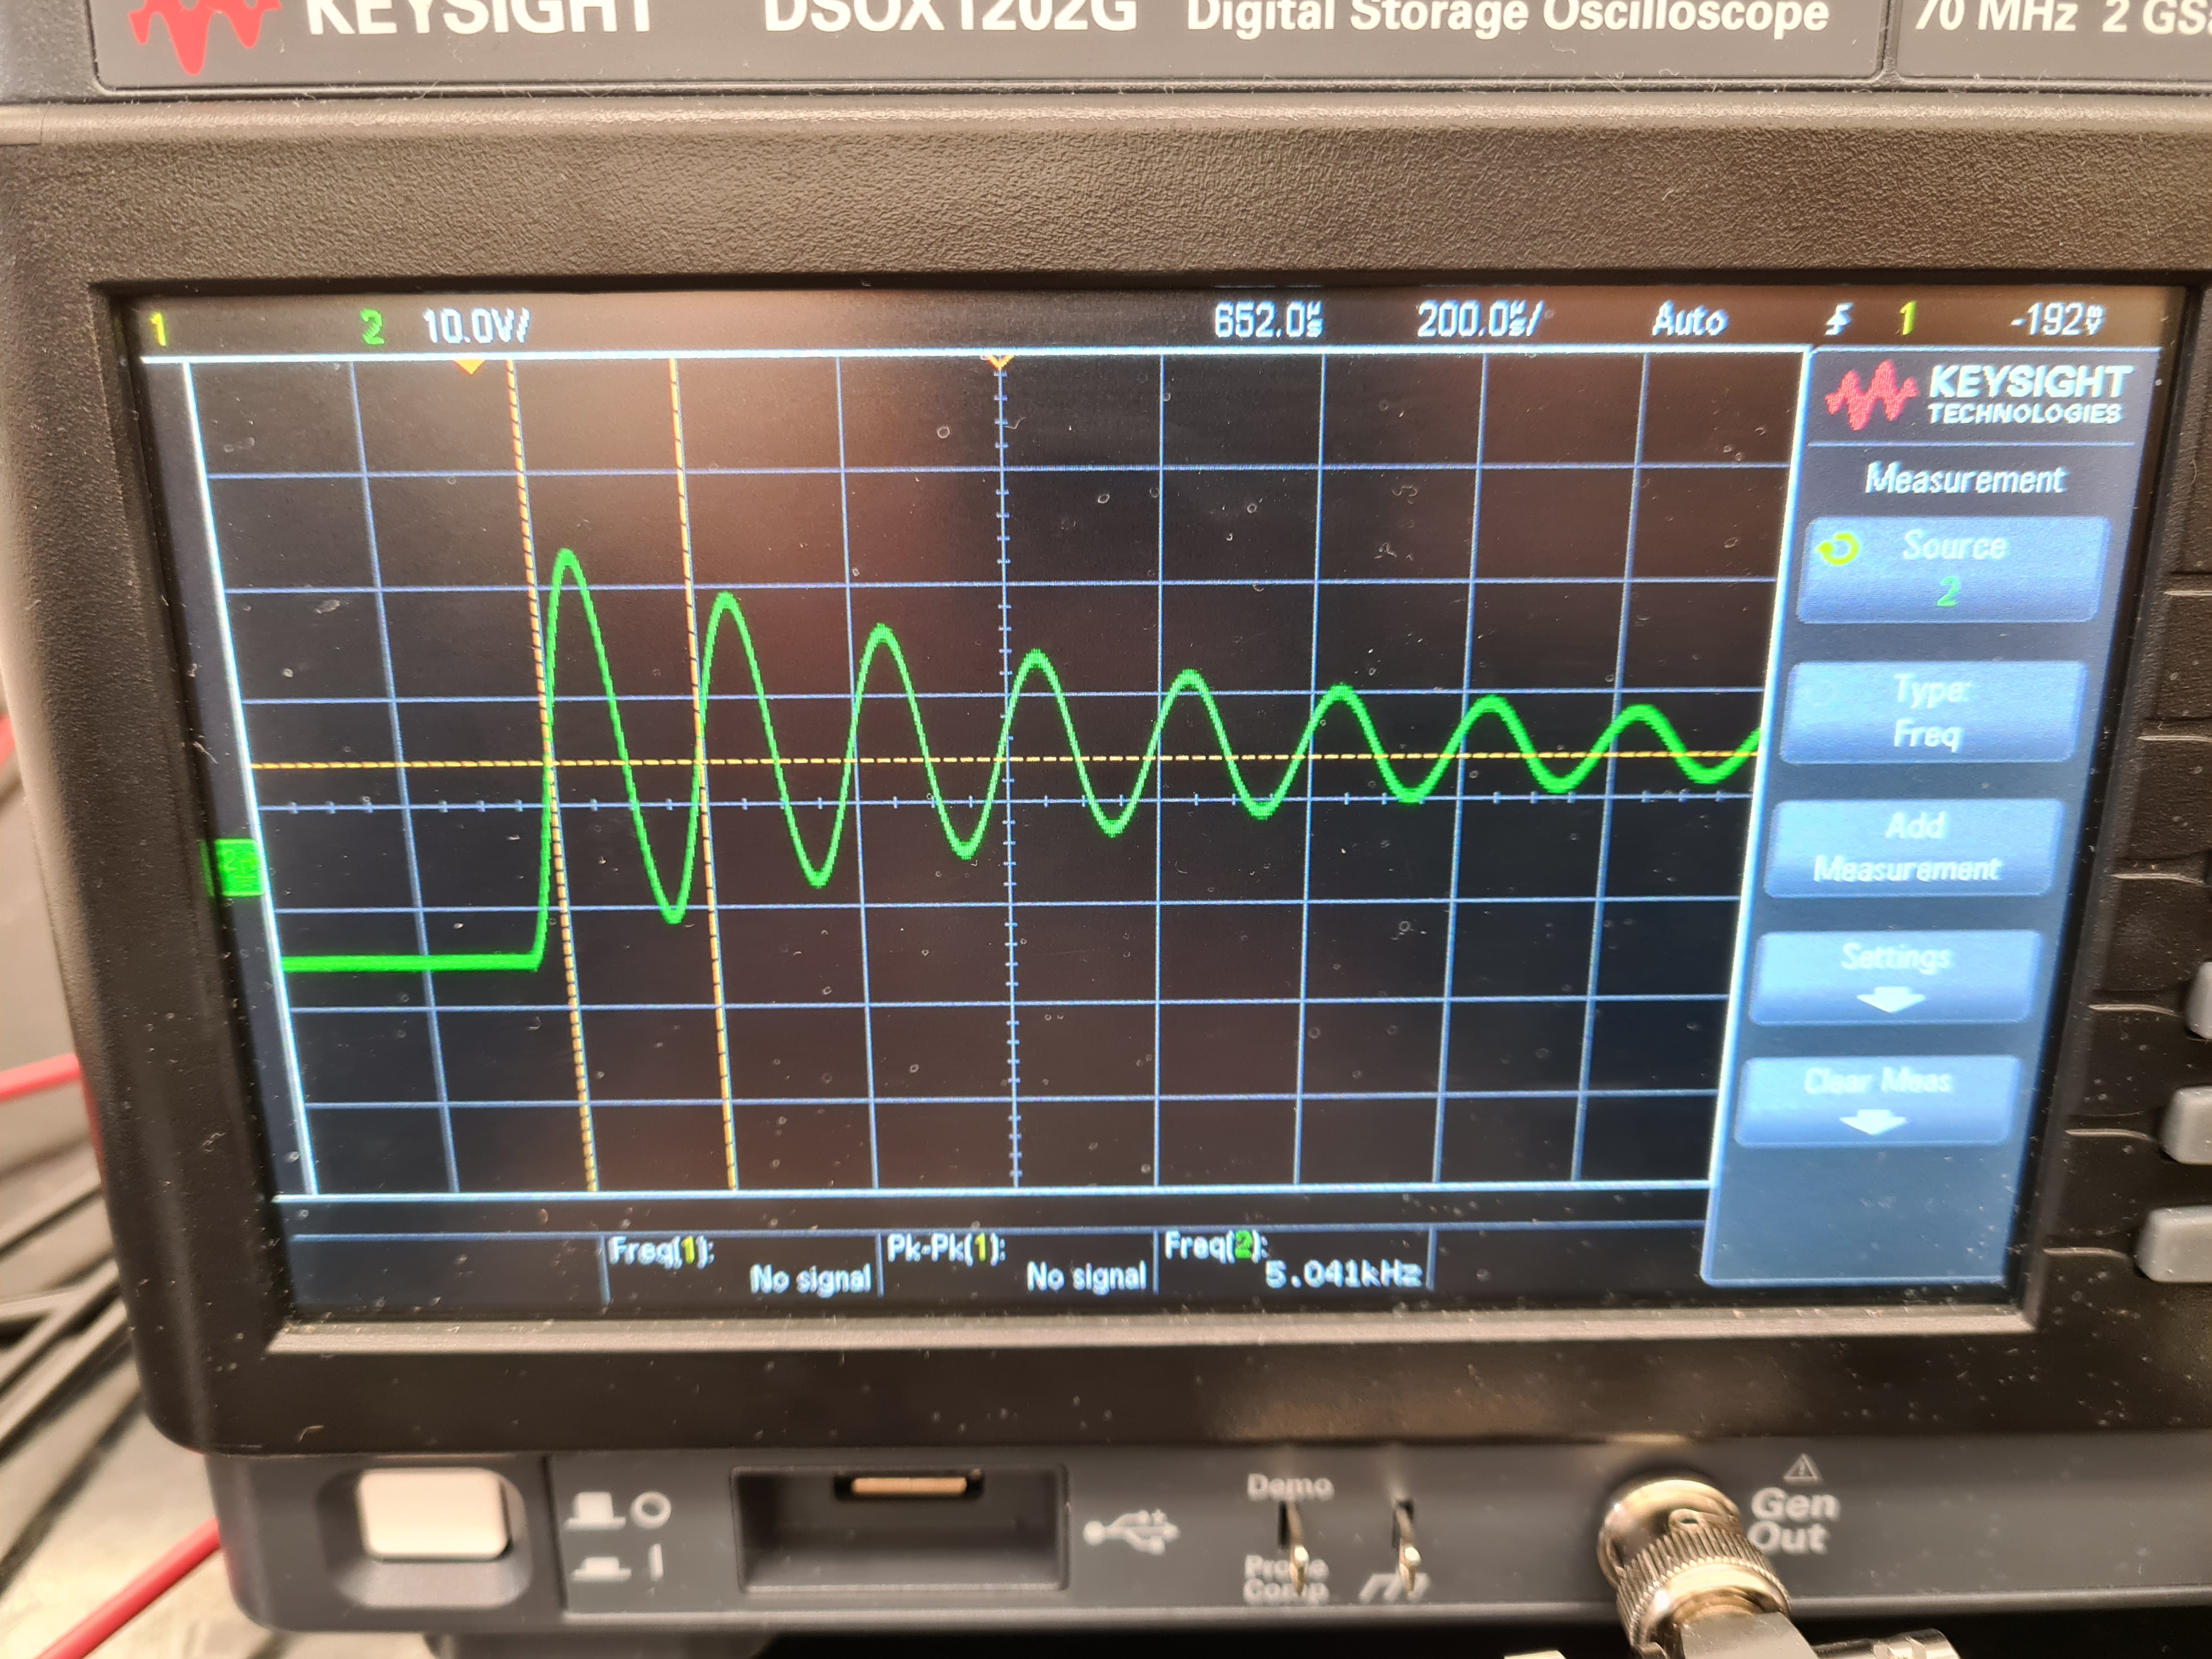
\includegraphics[width=0.9\linewidth]{../data/20211116_110834.jpg}
  \begin{center}
    \begin{center}   
    \end{center}  \end{center}
  \caption{Oscilloscope Reading (Peak to Peak Alignment)}
  \label{osc}
\end{figure}

\pagebreak

\subsection{Python Code}


\pagebreak

\begin{thebibliography}{99}

\bibitem{lab-manual-ex7} Currents in LCR - currents-l-c-r.pdf

\end{thebibliography}

\end{document}
